% Options for packages loaded elsewhere
% Options for packages loaded elsewhere
\PassOptionsToPackage{unicode}{hyperref}
\PassOptionsToPackage{hyphens}{url}
\PassOptionsToPackage{dvipsnames,svgnames,x11names}{xcolor}
%
\documentclass[
  french,
  9pt,
  a4paper,
]{article}
\usepackage{xcolor}
\usepackage[top = 3cm,bottom = 2.5cm,left = 2.5cm,right =
2.5cm]{geometry}
\usepackage{amsmath,amssymb}
\setcounter{secnumdepth}{3}
\usepackage{iftex}
\ifPDFTeX
  \usepackage[T1]{fontenc}
  \usepackage[utf8]{inputenc}
  \usepackage{textcomp} % provide euro and other symbols
\else % if luatex or xetex
  \usepackage{unicode-math} % this also loads fontspec
  \defaultfontfeatures{Scale=MatchLowercase}
  \defaultfontfeatures[\rmfamily]{Ligatures=TeX,Scale=1}
\fi
\usepackage{lmodern}
\ifPDFTeX\else
  % xetex/luatex font selection
\fi
% Use upquote if available, for straight quotes in verbatim environments
\IfFileExists{upquote.sty}{\usepackage{upquote}}{}
\IfFileExists{microtype.sty}{% use microtype if available
  \usepackage[]{microtype}
  \UseMicrotypeSet[protrusion]{basicmath} % disable protrusion for tt fonts
}{}
\usepackage{setspace}
\makeatletter
\@ifundefined{KOMAClassName}{% if non-KOMA class
  \IfFileExists{parskip.sty}{%
    \usepackage{parskip}
  }{% else
    \setlength{\parindent}{0pt}
    \setlength{\parskip}{6pt plus 2pt minus 1pt}}
}{% if KOMA class
  \KOMAoptions{parskip=half}}
\makeatother
% Make \paragraph and \subparagraph free-standing
\makeatletter
\ifx\paragraph\undefined\else
  \let\oldparagraph\paragraph
  \renewcommand{\paragraph}{
    \@ifstar
      \xxxParagraphStar
      \xxxParagraphNoStar
  }
  \newcommand{\xxxParagraphStar}[1]{\oldparagraph*{#1}\mbox{}}
  \newcommand{\xxxParagraphNoStar}[1]{\oldparagraph{#1}\mbox{}}
\fi
\ifx\subparagraph\undefined\else
  \let\oldsubparagraph\subparagraph
  \renewcommand{\subparagraph}{
    \@ifstar
      \xxxSubParagraphStar
      \xxxSubParagraphNoStar
  }
  \newcommand{\xxxSubParagraphStar}[1]{\oldsubparagraph*{#1}\mbox{}}
  \newcommand{\xxxSubParagraphNoStar}[1]{\oldsubparagraph{#1}\mbox{}}
\fi
\makeatother


\usepackage{longtable,booktabs,array}
\usepackage{calc} % for calculating minipage widths
% Correct order of tables after \paragraph or \subparagraph
\usepackage{etoolbox}
\makeatletter
\patchcmd\longtable{\par}{\if@noskipsec\mbox{}\fi\par}{}{}
\makeatother
% Allow footnotes in longtable head/foot
\IfFileExists{footnotehyper.sty}{\usepackage{footnotehyper}}{\usepackage{footnote}}
\makesavenoteenv{longtable}
\usepackage{graphicx}
\makeatletter
\newsavebox\pandoc@box
\newcommand*\pandocbounded[1]{% scales image to fit in text height/width
  \sbox\pandoc@box{#1}%
  \Gscale@div\@tempa{\textheight}{\dimexpr\ht\pandoc@box+\dp\pandoc@box\relax}%
  \Gscale@div\@tempb{\linewidth}{\wd\pandoc@box}%
  \ifdim\@tempb\p@<\@tempa\p@\let\@tempa\@tempb\fi% select the smaller of both
  \ifdim\@tempa\p@<\p@\scalebox{\@tempa}{\usebox\pandoc@box}%
  \else\usebox{\pandoc@box}%
  \fi%
}
% Set default figure placement to htbp
\def\fps@figure{htbp}
\makeatother


% definitions for citeproc citations
\NewDocumentCommand\citeproctext{}{}
\NewDocumentCommand\citeproc{mm}{%
  \begingroup\def\citeproctext{#2}\cite{#1}\endgroup}
\makeatletter
 % allow citations to break across lines
 \let\@cite@ofmt\@firstofone
 % avoid brackets around text for \cite:
 \def\@biblabel#1{}
 \def\@cite#1#2{{#1\if@tempswa , #2\fi}}
\makeatother
\newlength{\cslhangindent}
\setlength{\cslhangindent}{1.5em}
\newlength{\csllabelwidth}
\setlength{\csllabelwidth}{3em}
\newenvironment{CSLReferences}[2] % #1 hanging-indent, #2 entry-spacing
 {\begin{list}{}{%
  \setlength{\itemindent}{0pt}
  \setlength{\leftmargin}{0pt}
  \setlength{\parsep}{0pt}
  % turn on hanging indent if param 1 is 1
  \ifodd #1
   \setlength{\leftmargin}{\cslhangindent}
   \setlength{\itemindent}{-1\cslhangindent}
  \fi
  % set entry spacing
  \setlength{\itemsep}{#2\baselineskip}}}
 {\end{list}}
\usepackage{calc}
\newcommand{\CSLBlock}[1]{\hfill\break\parbox[t]{\linewidth}{\strut\ignorespaces#1\strut}}
\newcommand{\CSLLeftMargin}[1]{\parbox[t]{\csllabelwidth}{\strut#1\strut}}
\newcommand{\CSLRightInline}[1]{\parbox[t]{\linewidth - \csllabelwidth}{\strut#1\strut}}
\newcommand{\CSLIndent}[1]{\hspace{\cslhangindent}#1}

\ifLuaTeX
\usepackage[bidi=basic]{babel}
\else
\usepackage[bidi=default]{babel}
\fi
% get rid of language-specific shorthands (see #6817):
\let\LanguageShortHands\languageshorthands
\def\languageshorthands#1{}


\setlength{\emergencystretch}{3em} % prevent overfull lines

\providecommand{\tightlist}{%
  \setlength{\itemsep}{0pt}\setlength{\parskip}{0pt}}



 


\makeatletter
\@ifpackageloaded{caption}{}{\usepackage{caption}}
\AtBeginDocument{%
\ifdefined\contentsname
  \renewcommand*\contentsname{Table des matières}
\else
  \newcommand\contentsname{Table des matières}
\fi
\ifdefined\listfigurename
  \renewcommand*\listfigurename{Graphiques}
\else
  \newcommand\listfigurename{Graphiques}
\fi
\ifdefined\listtablename
  \renewcommand*\listtablename{Tableaux}
\else
  \newcommand\listtablename{Tableaux}
\fi
\ifdefined\figurename
  \renewcommand*\figurename{\textbf{Graphique}}
\else
  \newcommand\figurename{\textbf{Graphique}}
\fi
\ifdefined\tablename
  \renewcommand*\tablename{\textbf{Tableau}}
\else
  \newcommand\tablename{\textbf{Tableau}}
\fi
}
\@ifpackageloaded{float}{}{\usepackage{float}}
\floatstyle{ruled}
\@ifundefined{c@chapter}{\newfloat{codelisting}{h}{lop}}{\newfloat{codelisting}{h}{lop}[chapter]}
\floatname{codelisting}{Listing}
\newcommand*\listoflistings{\listof{codelisting}{Liste des Listings}}
\captionsetup{labelsep=period}
\makeatother
\makeatletter
\makeatother
\makeatletter
\@ifpackageloaded{caption}{}{\usepackage{caption}}
\@ifpackageloaded{subcaption}{}{\usepackage{subcaption}}
\makeatother
\usepackage{bookmark}
\IfFileExists{xurl.sty}{\usepackage{xurl}}{} % add URL line breaks if available
\urlstyle{same}
\hypersetup{
  pdftitle={Une part des salaires dans la VA élévée en 2025 en France},
  pdfauthor={Xavier Timbeau},
  pdflang={fr},
  colorlinks=true,
  linkcolor={blue},
  filecolor={Maroon},
  citecolor={Blue},
  urlcolor={Blue},
  pdfcreator={LaTeX via pandoc}}


%%% title.tex we use to call other packages. Because this works
\usepackage{titlepic}
\usepackage{titling}
\usepackage{graphicx}
\usepackage{fontspec}
\usepackage{placeins}
\usepackage{graphbox}
\usepackage{tikz}
\usepackage{geometry}
\usepackage{xcolor}
\usepackage{amsmath}
\usepackage[some]{background}
\usepackage{lipsum}
\usepackage{caption}
\usepackage{datetime}
\usepackage{xstring}
\usepackage{blindtext}
\usepackage{scrlayer-scrpage}

\setmainfont{OpenSans}[
  UprightFont = {*-Regular},
  BoldFont = {*-Bold},
  BoldItalicFont = {*-BoldItalic},
  ItalicFont = {*-Italic},
  Path = {_extensions/ofce/wp/OpenSans/},
  Extension = {.ttf}
]
\setsansfont{OpenSans}[
  UprightFont = {*-Regular},
  BoldFont = {*-Bold},
  BoldItalicFont = {*-BoldItalic},
  ItalicFont = {*-Italic},
  Path = {_extensions/ofce/wp/OpenSans/},
  Extension = {.ttf}
]

\def\getYear#1{\StrLeft{#1}{4}}
\def\getMonth#1{\StrMid{#1}{6}{7}}
\def\getDay#1{\StrRight{#1}{2}}

\def\jolimois#1{\monthname{\getMonth{#1}}}

\definecolor{quarto-callout-color}{HTML}{eeeeee}
\definecolor{quarto-callout-tip-color}{HTML}{dddddd}
\definecolor{quarto-callout-tip-color-frame}{HTML}{eeeeee}

\clearpairofpagestyles

\KOMAoptions{headsepline=true}

\pagestyle{scrheadings}
\setkomafont{pageheadfoot}{\small}

\rehead{Document de travail n°-xx}
\lohead{\includegraphics[height=0.25cm]{\_extensions/ofce/wp/ofce\_m.png}}

\lofoot*{\thepage}
\refoot*{\thepage}
\begin{document}



\definecolor{ofcepbbleu}{RGB}{1, 97, 131}
\definecolor{ofcerouge}{RGB}{198, 45, 43}
\definecolor{scporouge}{RGB}{231, 0, 26}

\begin{titlepage}
  \backgroundsetup{
    scale=1,
    angle=0,
    opacity=1,
    contents={
  \begin{tikzpicture}[remember picture,overlay]
    \useasboundingbox (0,0) rectangle(\the\paperwidth,\the\paperheight);
      \node [anchor = center] at (-2.875-5.25,12.5) {\includegraphics[width=2.5cm]{\_extensions/ofce/wp/ofce\_m.png}};
      \node [anchor = center] at (-2.875-5.25,-12.75){
\includegraphics[width=2.5cm]{\_extensions/ofce/wp/sciencespo.png}};
      \node [anchor = east] at (8.5,-11.5){\textcolor{black}{Publié le : 2025-09-08}};
      \node [anchor = east] at (8.5,-12){\textcolor{black}{Modifié le : 2025-10-02}};
      \node [anchor = east] at (8.5,13-0.7){\textcolor{gray}{\Huge\textit{Working Paper}}};
      \draw [thick,black](-5.75,-13) -- (-5.75,13);
      \draw [color = white, fill=ofcepbbleu] (8.7,11.4) rectangle (10.45,13.15);
      \draw [color = white, fill=ofcepbbleu, very thick] (8.75-.5,11.25-.5) rectangle (8.75+.6,11.25+.6);
      \node [anchor = east] at (11-0.7,13-0.7){\textcolor{white}{\huge\textbf{xx}}};
      \node [anchor = east] at (10-0.74,12-0.67){\textcolor{white}{\textbf{}}};
    \end{tikzpicture}
  }
}
\BgThispage

\hspace{4cm}
\begin{minipage}{12.5cm}
  \vspace{5cm}
  \begin{flushleft}
    \begin{spacing}{2.5}
      \textcolor{scporouge}{\Huge\textbf{\textsf{Une part des salaires
dans la VA élévée en 2025 en France}}}
    \end{spacing}
   \vspace{5mm}
  \textcolor{scporouge}{\large\textbf{\textsf{Comparaisons
internationales de 30~ans de partage de la valeur ajoutée}}}
 \vspace{5mm}
    \vspace{20mm}
  \end{flushleft}
  
    
   \textbf{Xavier Timbeau},           OFCE, Sciences Po Paris
   
  % by-author
 \end{minipage}


%%
%% deuxieme page
\newpage
\pagestyle{empty}
\raisebox{-22cm}{
    \begin{minipage}[b]{40em}
      \textcolor{scporouge}{
        \textbf{CONTACT}}{

          \vspace{0.2cm}
          \vspace{0.2cm}
        
        \textbf{OFCE} 
  
        10 place de Catalogne 
        
        75014 Paris, FRANCE 
        
        Tel : +33 1 44 18 54 24
        
        \url{https://www.ofce.sciences-po.fr}
      }
    \end{minipage}
}
%%
%%
\newpage
%% troisieme page
\pagestyle{empty}
%%  \raisebox{3cm}{\begin{minipage}{\linewidth}
%%  \includegraphics[width=2cm]{\_extensions/ofce/wp/ofce\_m.png}
%%
%%  
\includegraphics[width=2cm]{\_extensions/ofce/wp/sciencespo.png}
%%  \end{minipage}}
%%
 
\LARGE\textbf{Une part des salaires dans la VA élévée en 2025 en France}

\large\textbf{Comparaisons internationales de 30~ans de partage de la
valeur ajoutée}

\vspace{1cm}


\par\rule{\textwidth}{0.5pt}

On explore ici différentes façons de calculer la notion de part des
salaires dans la valeur ajoutée. Le concept privilégié est celui de la
part des salaires \emph{corrigés de la non salarisation} dans la valeur
ajoutée \emph{nette de la consommation de capital fixe} des branches
\emph{marchandes hors services immobiliers des ménages}. Il peut être
calculé pour les pays européens. Il fait apparaître une position
singulière de la France où la part des salaires est plus élevé et s'est
accrue de façon importante. Bien que plus fragile empiriquement, la
notion de rendement du capital productif confirme ce diagnostic et
illustre un problème particulerement préoccupant du tissu productif
français. L'ensemble des éléments présentés ici est reproductible à
partir des codes fournis.3830 mots.

\par\rule{\textwidth}{0.5pt}


\vspace{1cm}

\begin{flushright}
   \linespread{1}\small{\textbf{Xavier
Timbeau}}, {\small{xavier.timbeau@sciencespo.fr}}\par
 % by-author
\end{flushright}
\end{titlepage}
\renewcommand*\contentsname{Table des matières}
{
\hypersetup{linkcolor=}
\setcounter{tocdepth}{1}
\tableofcontents
}

\setstretch{1.25}
\section{Du partage de la VA au partage des
richesses}\label{du-partage-de-la-va-au-partage-des-richesses}

L'analyse du partage de la valeur ajoutée (graphique~\ref{fig-psal}) est
au cœur des débats sur la redistribution des richesses (voir notamment
Hurlin et Portier (1996), Timbeau (2002), Cotis (2009), Husson (2010),
Askenazy, Cette et Sylvain (2012), Piton (2019), Timbeau (2025)). Un
indicateur souvent retenu est celui de la part des salaires dans la
valeur ajoutée. Nous discutons ici de la construction de cet indicateur
et de sa comparabilité entre pays (européens ou non).

\begin{figure}[H]

\caption{\label{fig-psal}Part des salaires dans la VA nette}

\centering{

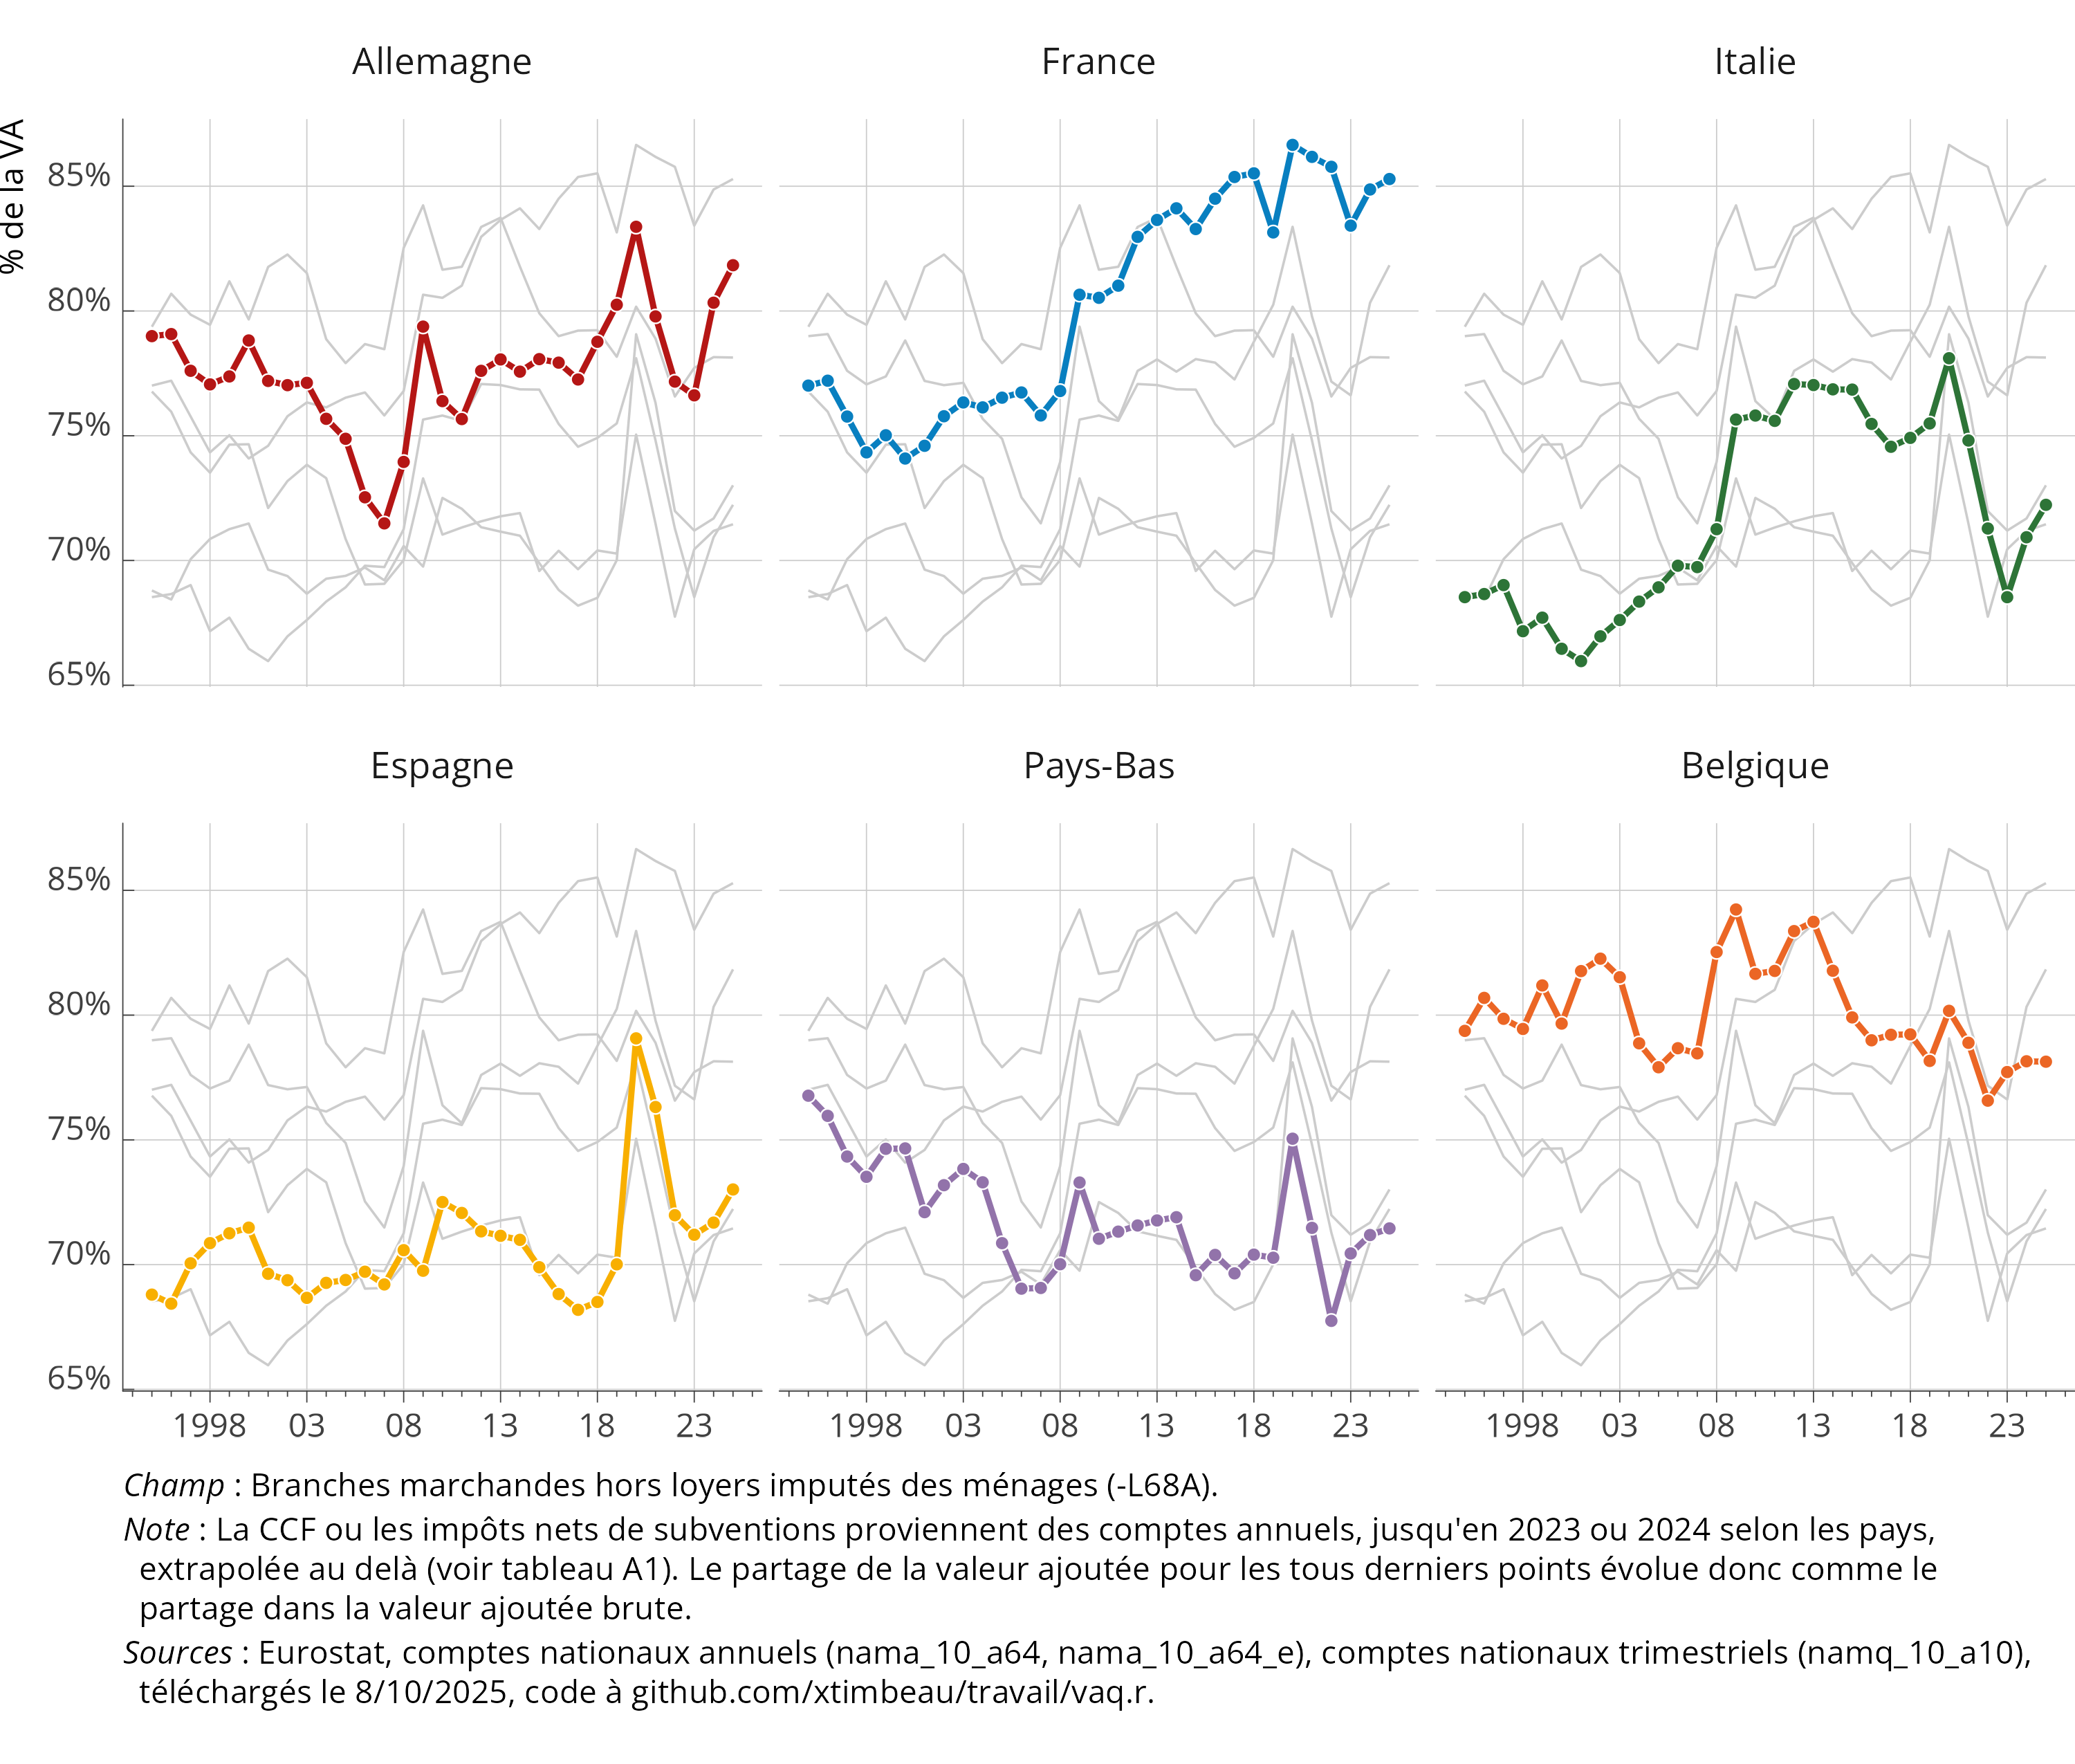
\includegraphics[width=1\linewidth,height=\textheight,keepaspectratio]{psal_comp_files/figure-pdf/fig-psal-1.png}

}

\end{figure}%

Trois points sont importants pour disposer du bon concept\,:

\begin{itemize}
\item
  Corriger des non salariés et leur imputer une masse salariale. Cette
  correction est standard. Elle repose sur des hypothèses importantes
  comme le salaire affecté à un non salarié. Nous utilisons la
  décomposition en branches (ou en secteurs dans certains pays) pour
  affecter aux non salariés d'une branche le salaire moyen des salariés
  de cette branche. C'est une hypothèse assez forte, mais qu'il est
  difficile de dépasser. Elle a des conséquences pour les comparaisons
  entre périodes pour un même pays parce que la part des non salariés
  varie dans le temps, de façon différente suivant les branches et entre
  pays.
\item
  Définir le champ considéré. Il est plus facile de faire le calcul au
  niveau le plus agrégé, mais ce champ inclut les branches non
  marchandes dans lesquelles la notion de prix et donc de valeur ajoutée
  est parfois conventionnelle. Parmi les branches marchandes, la
  branches des services immobiliers est problématique parce qu'elle
  prend en compte la valeur ajoutée des ménages au travers des services
  immobiliers qui sont pour par auto produit (les loyers imputés aux
  propriétaires). La notion de partage de la valeur ajoutée n'a ici pas
  beaucoup de sens et la comparaison d'un pays à l'autre peut être très
  perturbée. La notion privilégiée est donc celle de partage de la
  valeur ajoutée dans les branches marchandes hors services immobiliers
  des ménages ou, de façon plus précise, en enlevant de la valeur
  ajoutée marchande la sous branche «\,\emph{loyers imputés aux
  propriétaires occupants} (L68a)\,» et en considérant que la masse
  salariale et l'emploi salarié ou non salarié associés sont nuls.
\item
  Utiliser la notion de valeur ajoutée nette (de la consommation de
  capital fixe (CCF)) plutôt que brute. Rappelons que la valeur ajoutée
  nette est construite en ôtant de la valeur ajoutée brute la
  consommation de capital fixe. Cette dernière notion découle de
  l'application de tables de mortalité à un inventaire permanent des
  investissements non financiers (i.e.~les investissements physiques
  mais aussi ceux en logiciels ou en base de données ainsi que les
  investissements intangibles comme les marques). En traitant les
  investissements comme une consommation intermédiaire mesurée par leur
  amortissement physique ou fiscal, on est plus proche de la réalité du
  processus productif. Lorsque le taux de dépréciation du capital varie,
  par des changement dans les tables de mortalité, des changements dans
  la composition du capital ou des changements dans la structure par
  branche de l'économie, la CCF rapportée à la valeur ajoutée varie et
  modifie donc la perception des évolutions du partage de la valeur
  ajoutée. La notion de valeur ajoutée nette est meilleure pour des
  comparaisons dans l'espace ou dans le temps. Comme pour la correction
  pour les non salariés, la prise en compte de la valeur ajoutée nette
  modifie dans le temps et dans l'espace la part des salaires dans la
  valeur ajoutée.
\end{itemize}

Le concept que nous privilégions est donc défini comme suit (où, pour
chaque branche \(D1_b\) est la masse salariale chargée, \(B1G_b\) la
valeur ajoutée brute, \(P51C_b\) la \(CCF_b\), les trois notions en
euros aux prix courants et \(ns_b\) et \(sal_b\) les effectifs en
personne par branche)\,:

\[
s_{net, n.s., -L68AOQ}  = \frac{\sum_{b\in{TT-L68AOQ}}{D1_b*(1+ns_b/sal_b)}}{\sum_{b\in{TT-L68AOQ}}{B1G_b - P51C_b}}
\]

La part des salaires dans la valeur ajoutée nette est croissante en
France (graphique~\ref{fig-psal}) (de 10~points de 1998 à 2025), comme
en Espagne (de 9~points). Elle atteint en France le niveau le plus élevé
des pays sélectionnés, pour autant que l'on puisse comparer entre pays.

Théoriquement, l'évolution de part des salaires dans la valeur ajoutée
dépend de la fonction de production agrégée (ce qui suppose qu'elle
existe). Si l'élasticité de substitution entre le capital et la travail
est unitaire alors on s'attend à ce que le partage soit indépendant du
prix relatif du travail et du capital. La part des salaires est alors
uniquement déterminée par la forme de la fonction de production et
devrait converger dans tous les pays vers une valeur semblable, par
diffusion de la technologie. Une structure de l'économie par branche
différente peut cependant se traduire par des parts différentes d'un
pays à l'autre.

L'élasticité estimée généralement, au moins à moyen terme, est
sensiblement inférieure à 1, en tout cas sur données macroéconomique.
Cela implique qu'une hausse du prix du travail relativement par au
capital se traduit par une hausse de la part du travail dans la valeur
ajoutée\,-- la réciproque étant bien entendu vraie si c'est le capital
qui est relativement plus cher. Cela peut conduire à des variations plus
persistantes de la part des salaires dans la valeur ajoutée, mais ces
variations doivent reproduire celles des prix relatifs.

La part des salaires dans la valeur ajoutée est la plus basse aux
Pays-Bas et est sur une pente décroissante depuis plus de 20~ans, alors
qu'elle semble stable en Belgique et en Allemagne. L'Italie affiche une
variabilité temporelle importante, avec un pic de la part des salaires
dans la valeur ajoutée en 2013, puis une franche décroissance (de plus
de 13~points) interrompue dans la période récente suite à la période
d'inflation et la forte relance budgétaire.

En France, la hausse est franche après la crise financière de 2008,
suivant une période de grande stabilité de 1995 à 2007. Cette hausse
peut découler d'un effet de structure sectorielle, mais le
graphique~\ref{fig-salaires} indique une autre singularité française.
Contrairement à de nombreux pays, les salaires réels sont restés sur une
pente croissante, interrompue par la phase d'inflation à partir de la
fin de l'année 2021, alors que dans les 5 autres pays, 2008 marque une
cassure dans la progression de salaires réels.

Depuis 2018, en France, la part des salaires est stabilisée, à un haut
niveau (graphique~\ref{fig-psal}). L'inflation et le retard d'ajustement
des salaires sur l'inflation explique probablement cette trajectoire. On
observe des mouvements comparables dans d'autres pays, bien que plus
violent en Allemagne ou en Italie par exemple.

Au début des années 2000, deux pays se distinguaient des autres
(l'Espagne et l'Italie) par une part des salaires plus faibles. L'écart
avec l'Allemagne atteignait alors plus de 15~points. En généralisant
l'approche aux pays de l'Union Européenne, on peut en partie confirmer
cette hypothèse (graphique~\ref{fig-psaleu}). Les pays qui ont connu un
développement rapide, et donc des niveaux d'investissement élevés, on eu
des parts des salaires basses (La Bulgarie, la Tchéquie, la Grèce par
exemple). Mais ce n'est pas une observation systématique\,: certains
pays moins développés ont eu par le passé une part très élevée des
salaires dans la valeur ajouté, témoignant peut être de modes de
formation des salaires et d'inflation particulier et hérités du passé.
Cependant, comme le suggèrent la position singulière de quelques petits
pays, parmi lesquels l'Irlande, le Luxembourg, Malte, Chypre ou les
Pays-Bas dans une certaine mesure, c'est peut être du côté du
déplacement de la base imposable des profits (optimisation fiscale), des
prix de transferts et d'une position très particulière dans la chaîne de
valeur qu'il faut aller chercher l'explication de très faibles parts des
salaires dans la valeur ajoutée.

\begin{figure}[H]

\caption{\label{fig-psaleu}Part des salaires dans la VA nette 1995 et
2025}

\centering{

\subcaption{\label{fig-psaleu-1}Part des salaires dans la VA nette 1995
et 2025 VA nette}

\centering{

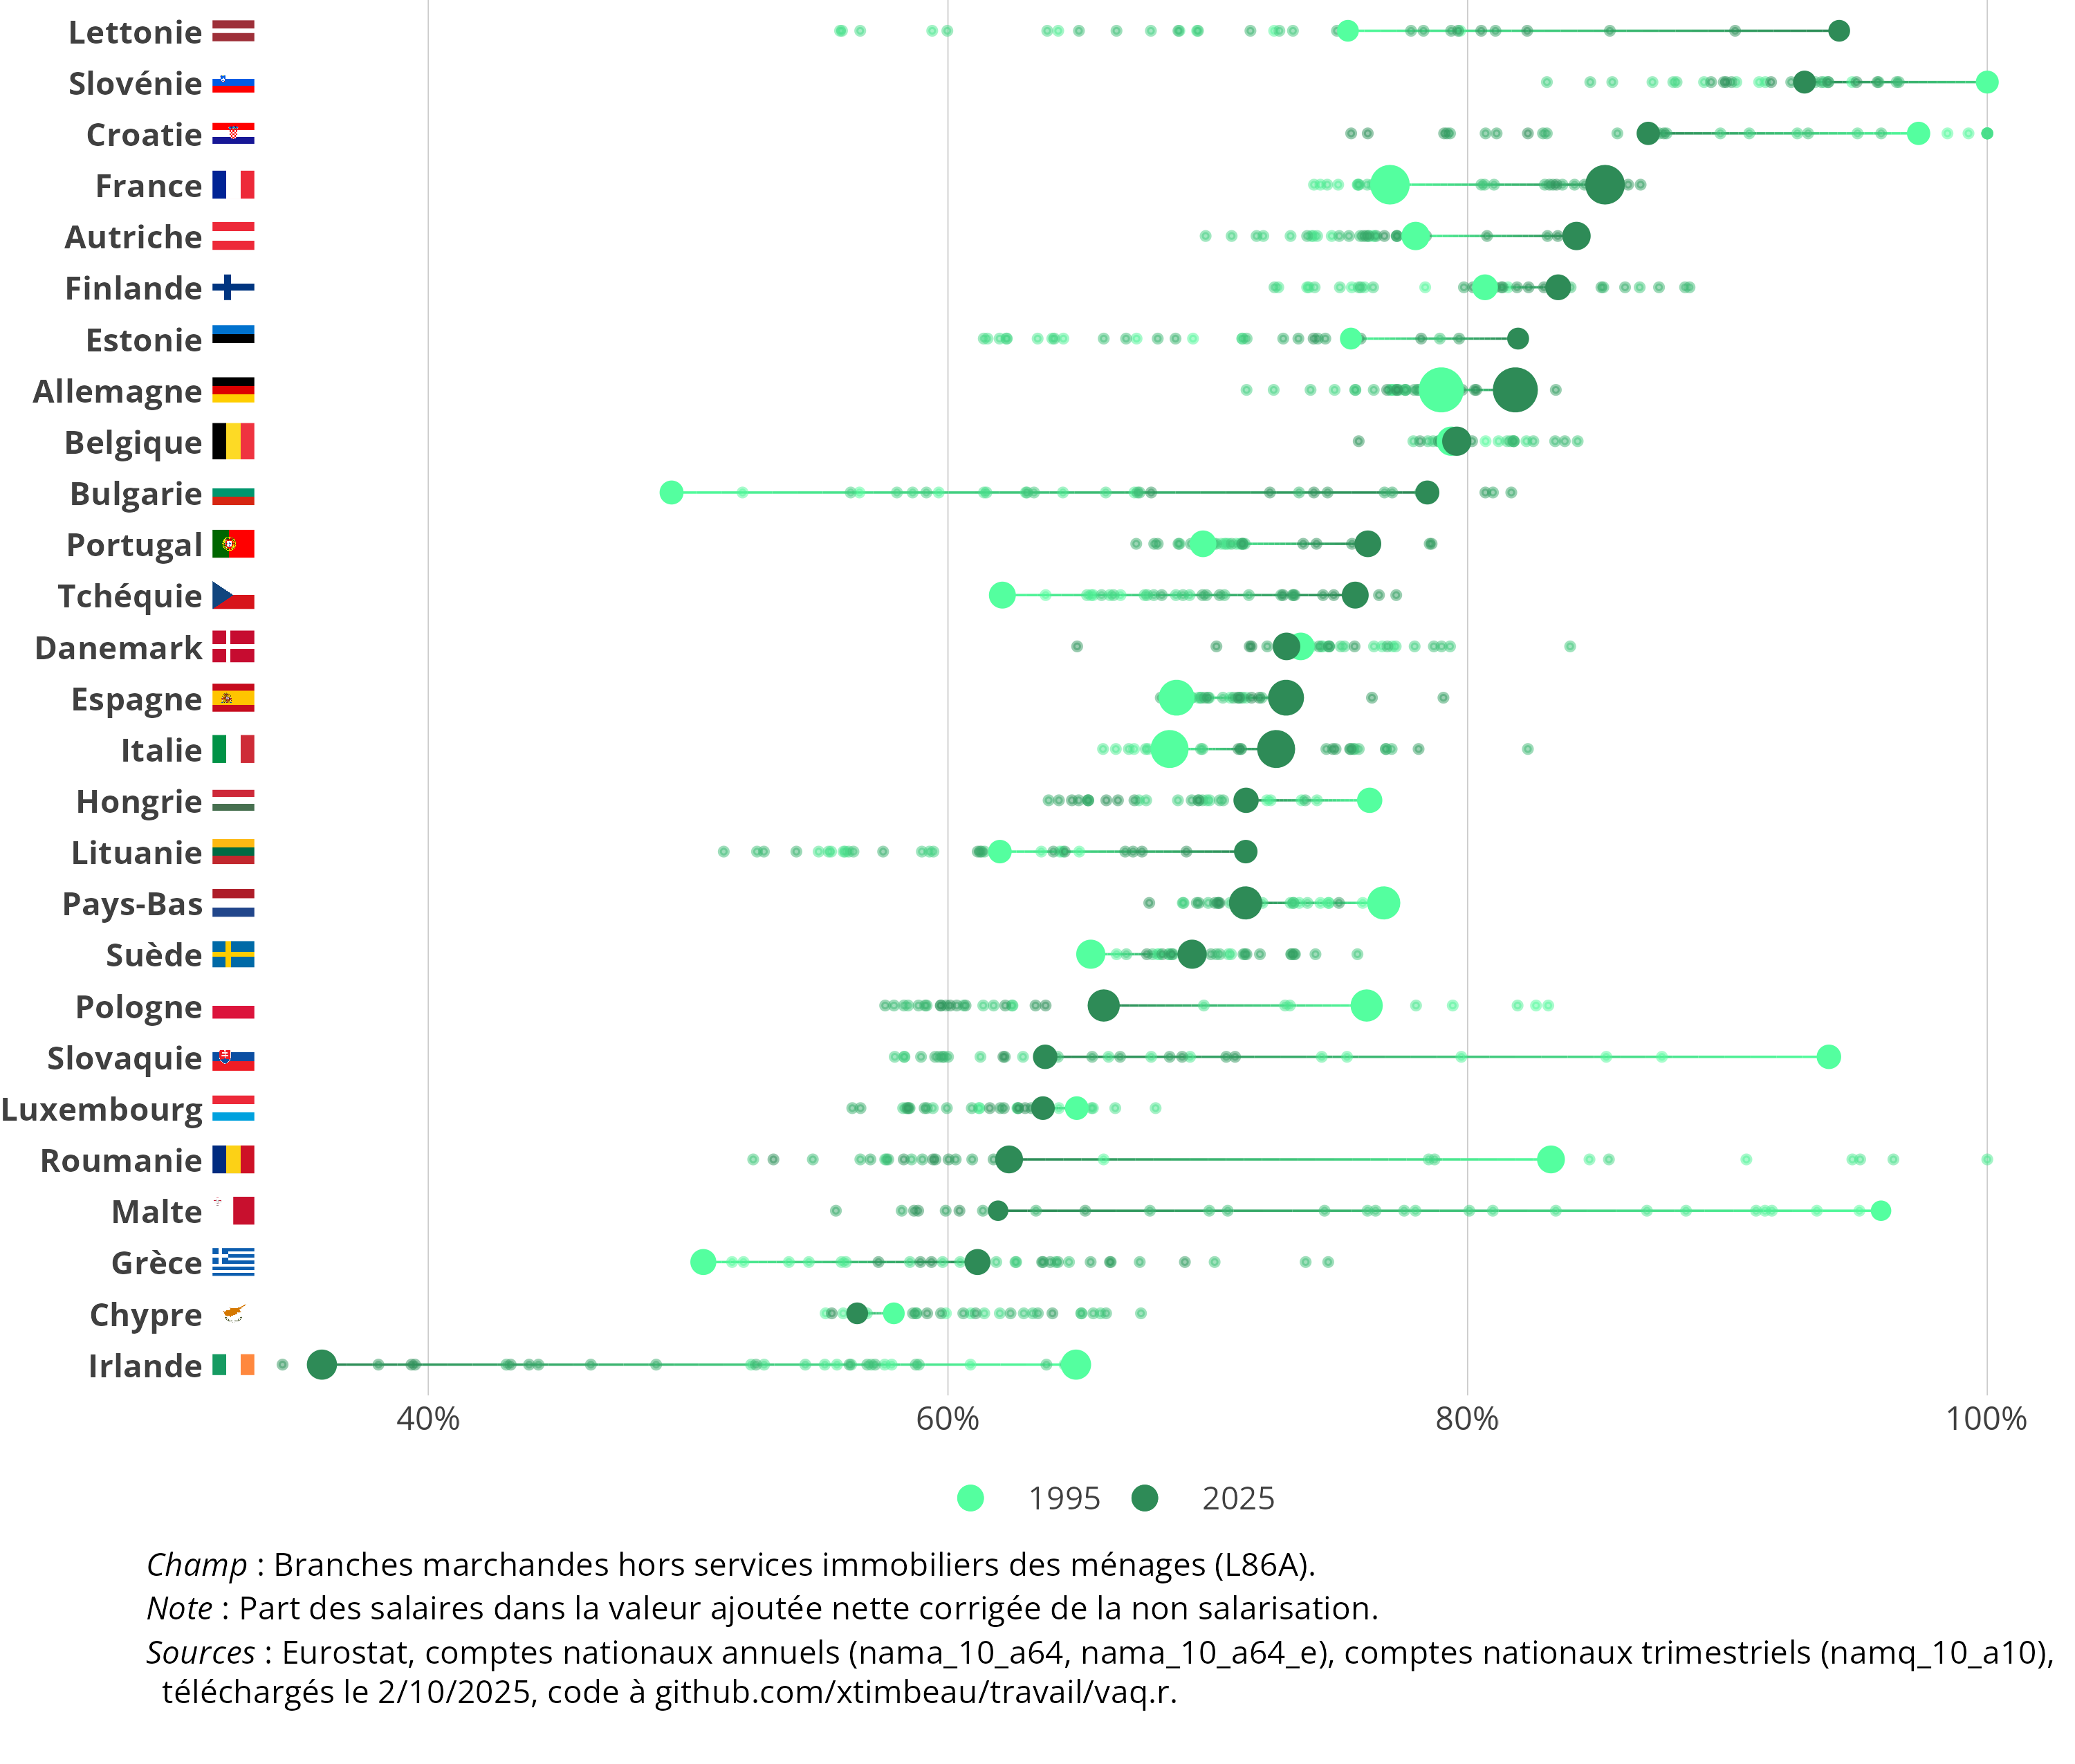
\includegraphics[width=1\linewidth,height=\textheight,keepaspectratio]{psal_comp_files/figure-pdf/fig-psaleu-1-1.png}

}

}

\end{figure}%

La construction d'un taux de rendement du capital est sans doute assez
fragile parce qu'il faut ajouter à l'évaluation du partage de la valeur
ajoutée une estimation des impôts payés (notamment l'impôt sur les
sociétés) et une évaluation du stock de capital. En utilisant les
données de stock de capital productif le diagnostic présenté sur le
graphique~\ref{fig-psal} est confirmé par le graphique~\ref{fig-rp}. La
France y occupe une position singulière avec un rendement du capital
productif particulièrement faible et décroissant depuis le début des
années 2000 alors qu'il est constant dans beaucoup de pays ou même
croissant comme aux Pays-Bas. Une explication possible est le
déplacement de la base fiscale en Europe comme le suggèrent Tørsløv,
Wier et Zucman (2022).

\begin{figure}[H]

\caption{\label{fig-rp}Rendement du capital productif}

\centering{

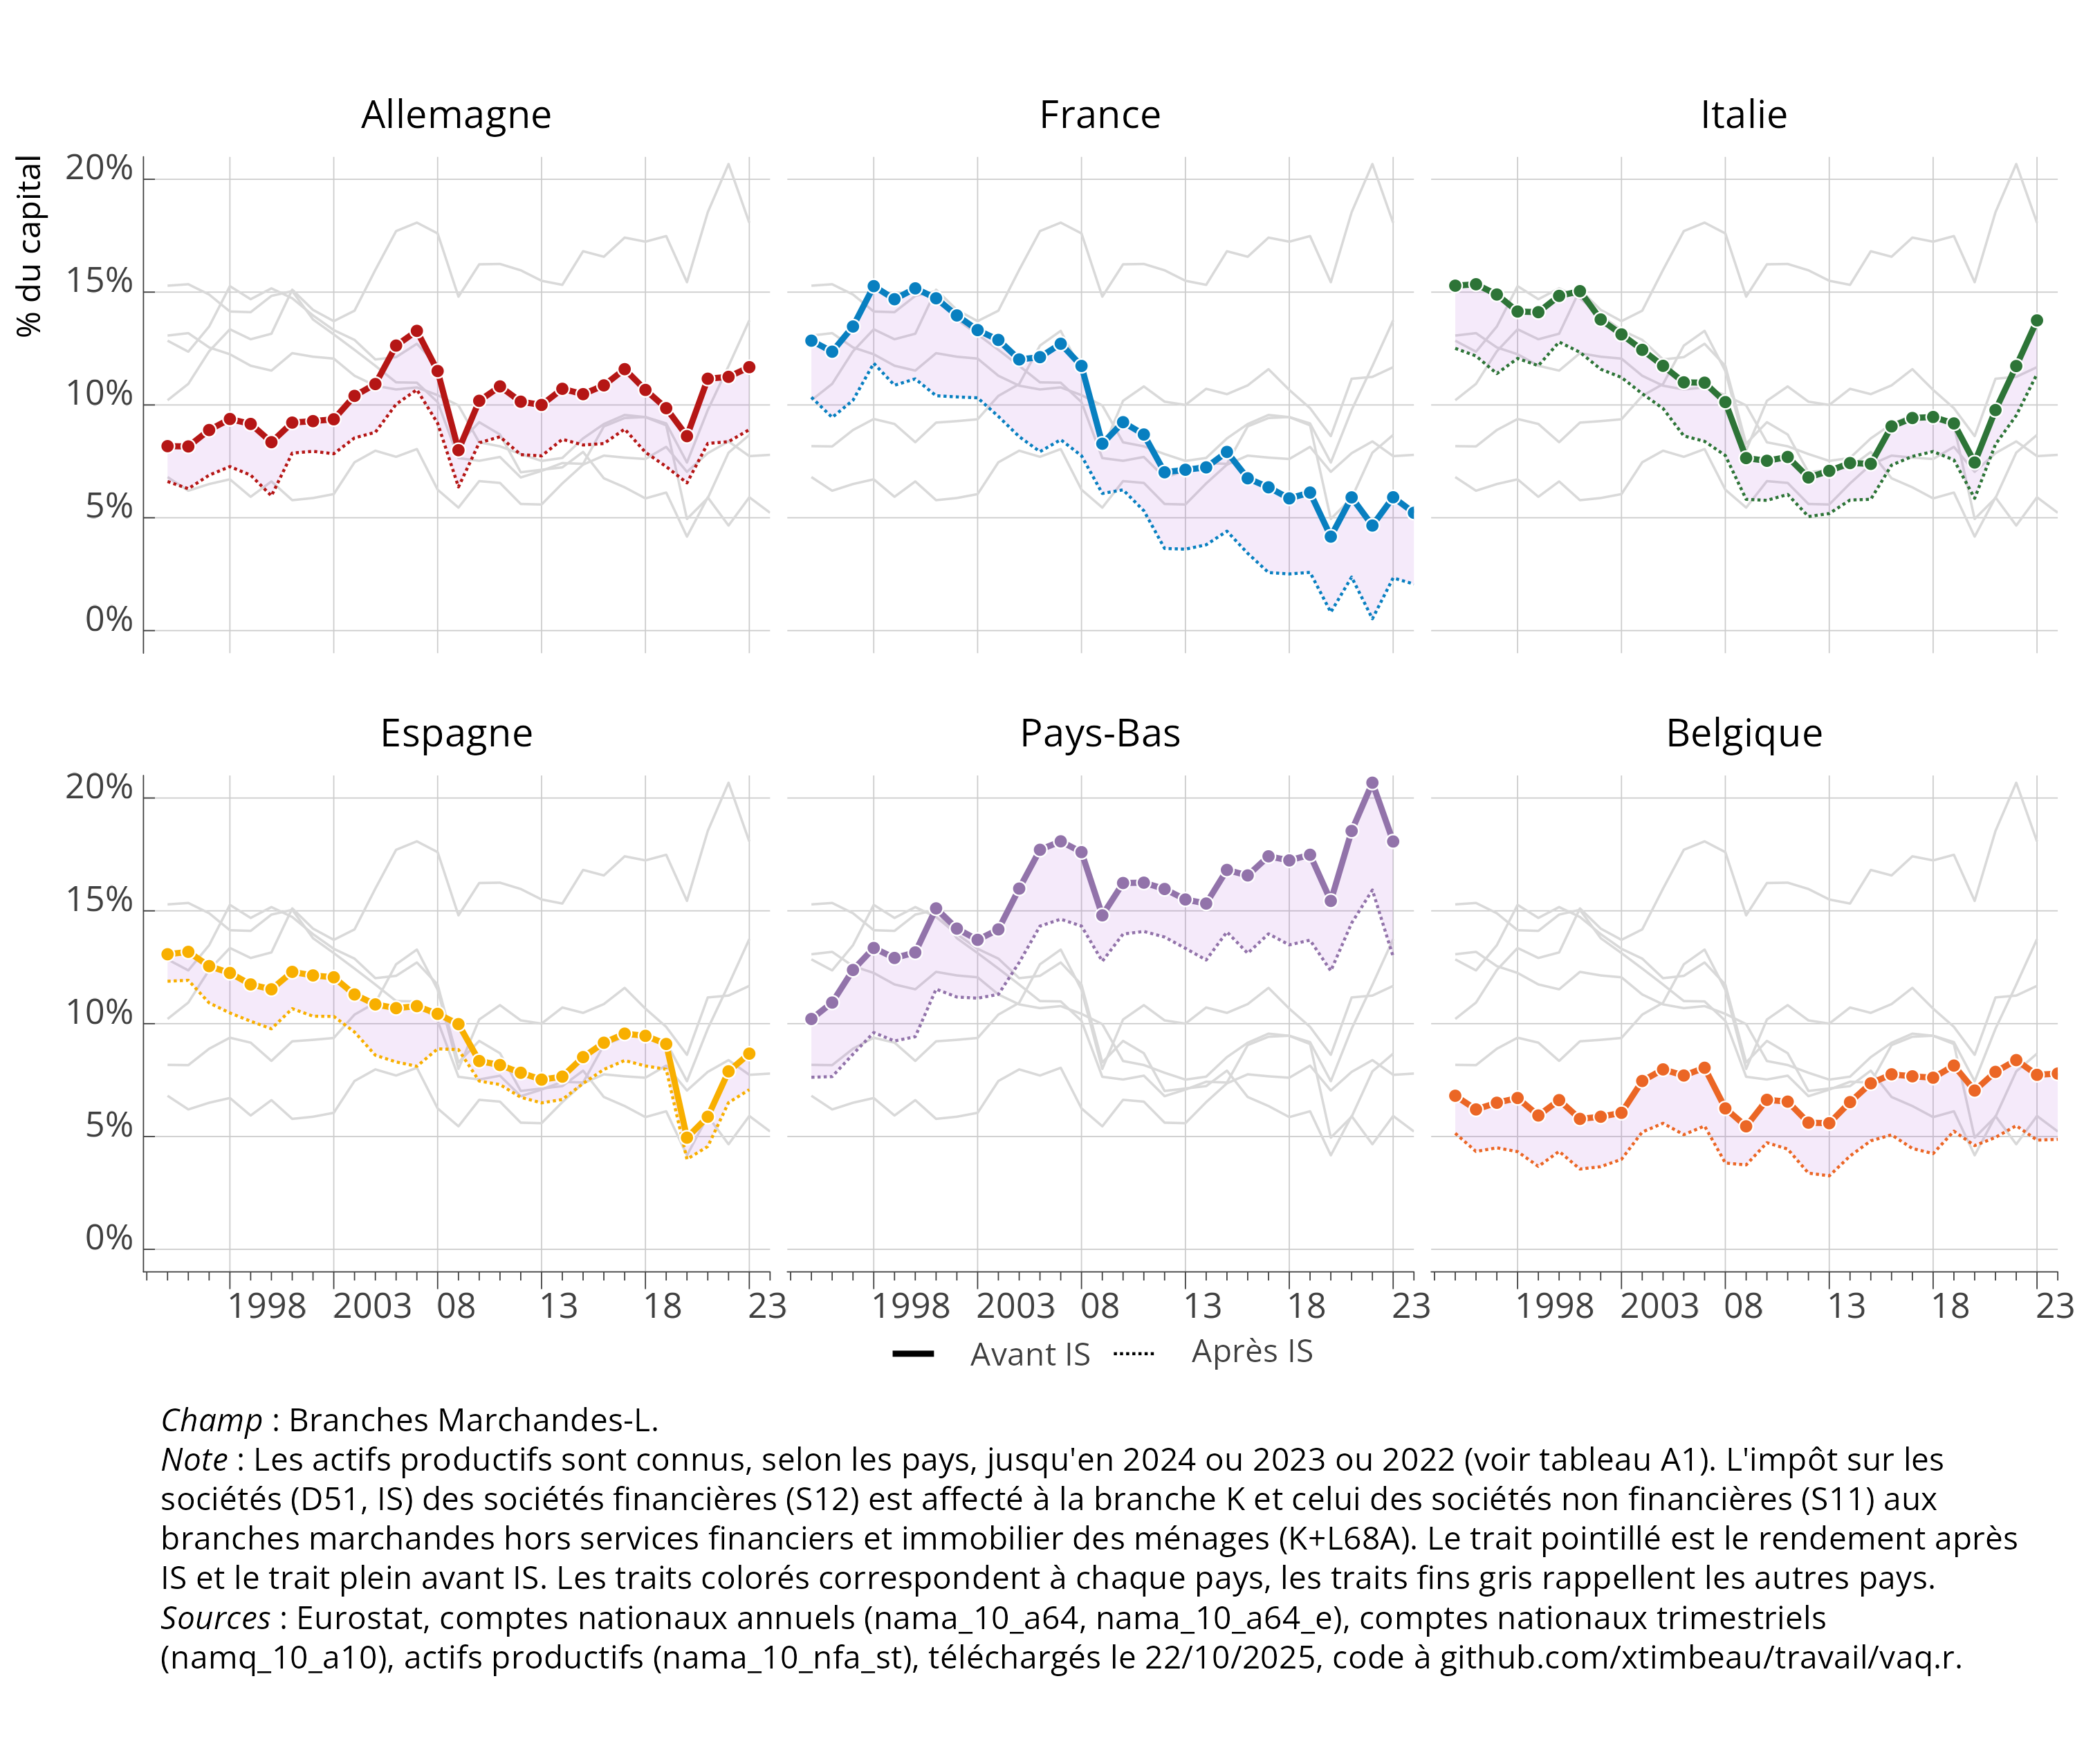
\includegraphics[width=1\linewidth,height=\textheight,keepaspectratio]{psal_comp_files/figure-pdf/fig-rp-1.png}

}

\end{figure}%

On détaille en les discutant dans la suite de ce document les effets des
corrections appliquées, ainsi que la différence entre les mesures
dérivées des comptes de branche ou des comptes d'agents. Ces éléments
sont un peu fastidieux, mais ils s'avèrent assez importants et pas
toujours très intuitifs.

On explore également les conséquences en matière de taux de profit (part
des profits nets dans la valeur ajoutée) ou rendement du capital
(profits nets divisés par les actifs).

\section{Evolution des salaires
réels}\label{evolution-des-salaires-ruxe9els}

L'évolution des salaries réels est un complément à celle du partage de
la valeur ajoutée. Pour passer de l'un à l'autre, il faut non seulement
prendre en compte les évolutions de la valeur ajoutée, mais aussi les
effets de l'évolution du ratio prix à la consommation sur prix de valeur
ajoutée.

On déflate la masse salariale (comptabilité nationale, comptes
trimestriels) par les prix à la consommation. On utilise les masses
salariales (\(D1\), dans
\href{https://ec.europa.eu/eurostat/databrowser/view/NAMQ_10_A10/default/table?lang=en}{\texttt{namq\_10\_a10}})
par branches pour comparer branches (principalement) marchandes et
(principalement) non marchandes divisées par l'emploi salarié
(\href{https://ec.europa.eu/eurostat/databrowser/view/NAMQ_10_A10_E__custom_7475124/default/table?lang=en}{\texttt{namq\_10\_a10\_e}}).
Les prix sont les déflateurs de la consommation (\(P31\_S14\) dans
\href{https://ec.europa.eu/eurostat/databrowser/product/page/NAMQ_10_FCS}{\texttt{namq\_10\_fcs}})
chaînés (voir le code pour les détails).

On distingue 4 agrégations\,: l'ensemble des branches (ou l'ensemble de
l'économie), les branches non marchandes, les branches marchandes et les
branches marchandes hors immobilier.

\begin{figure}[H]

\caption{\label{fig-salaires}Salaires réels en Europe}

\centering{

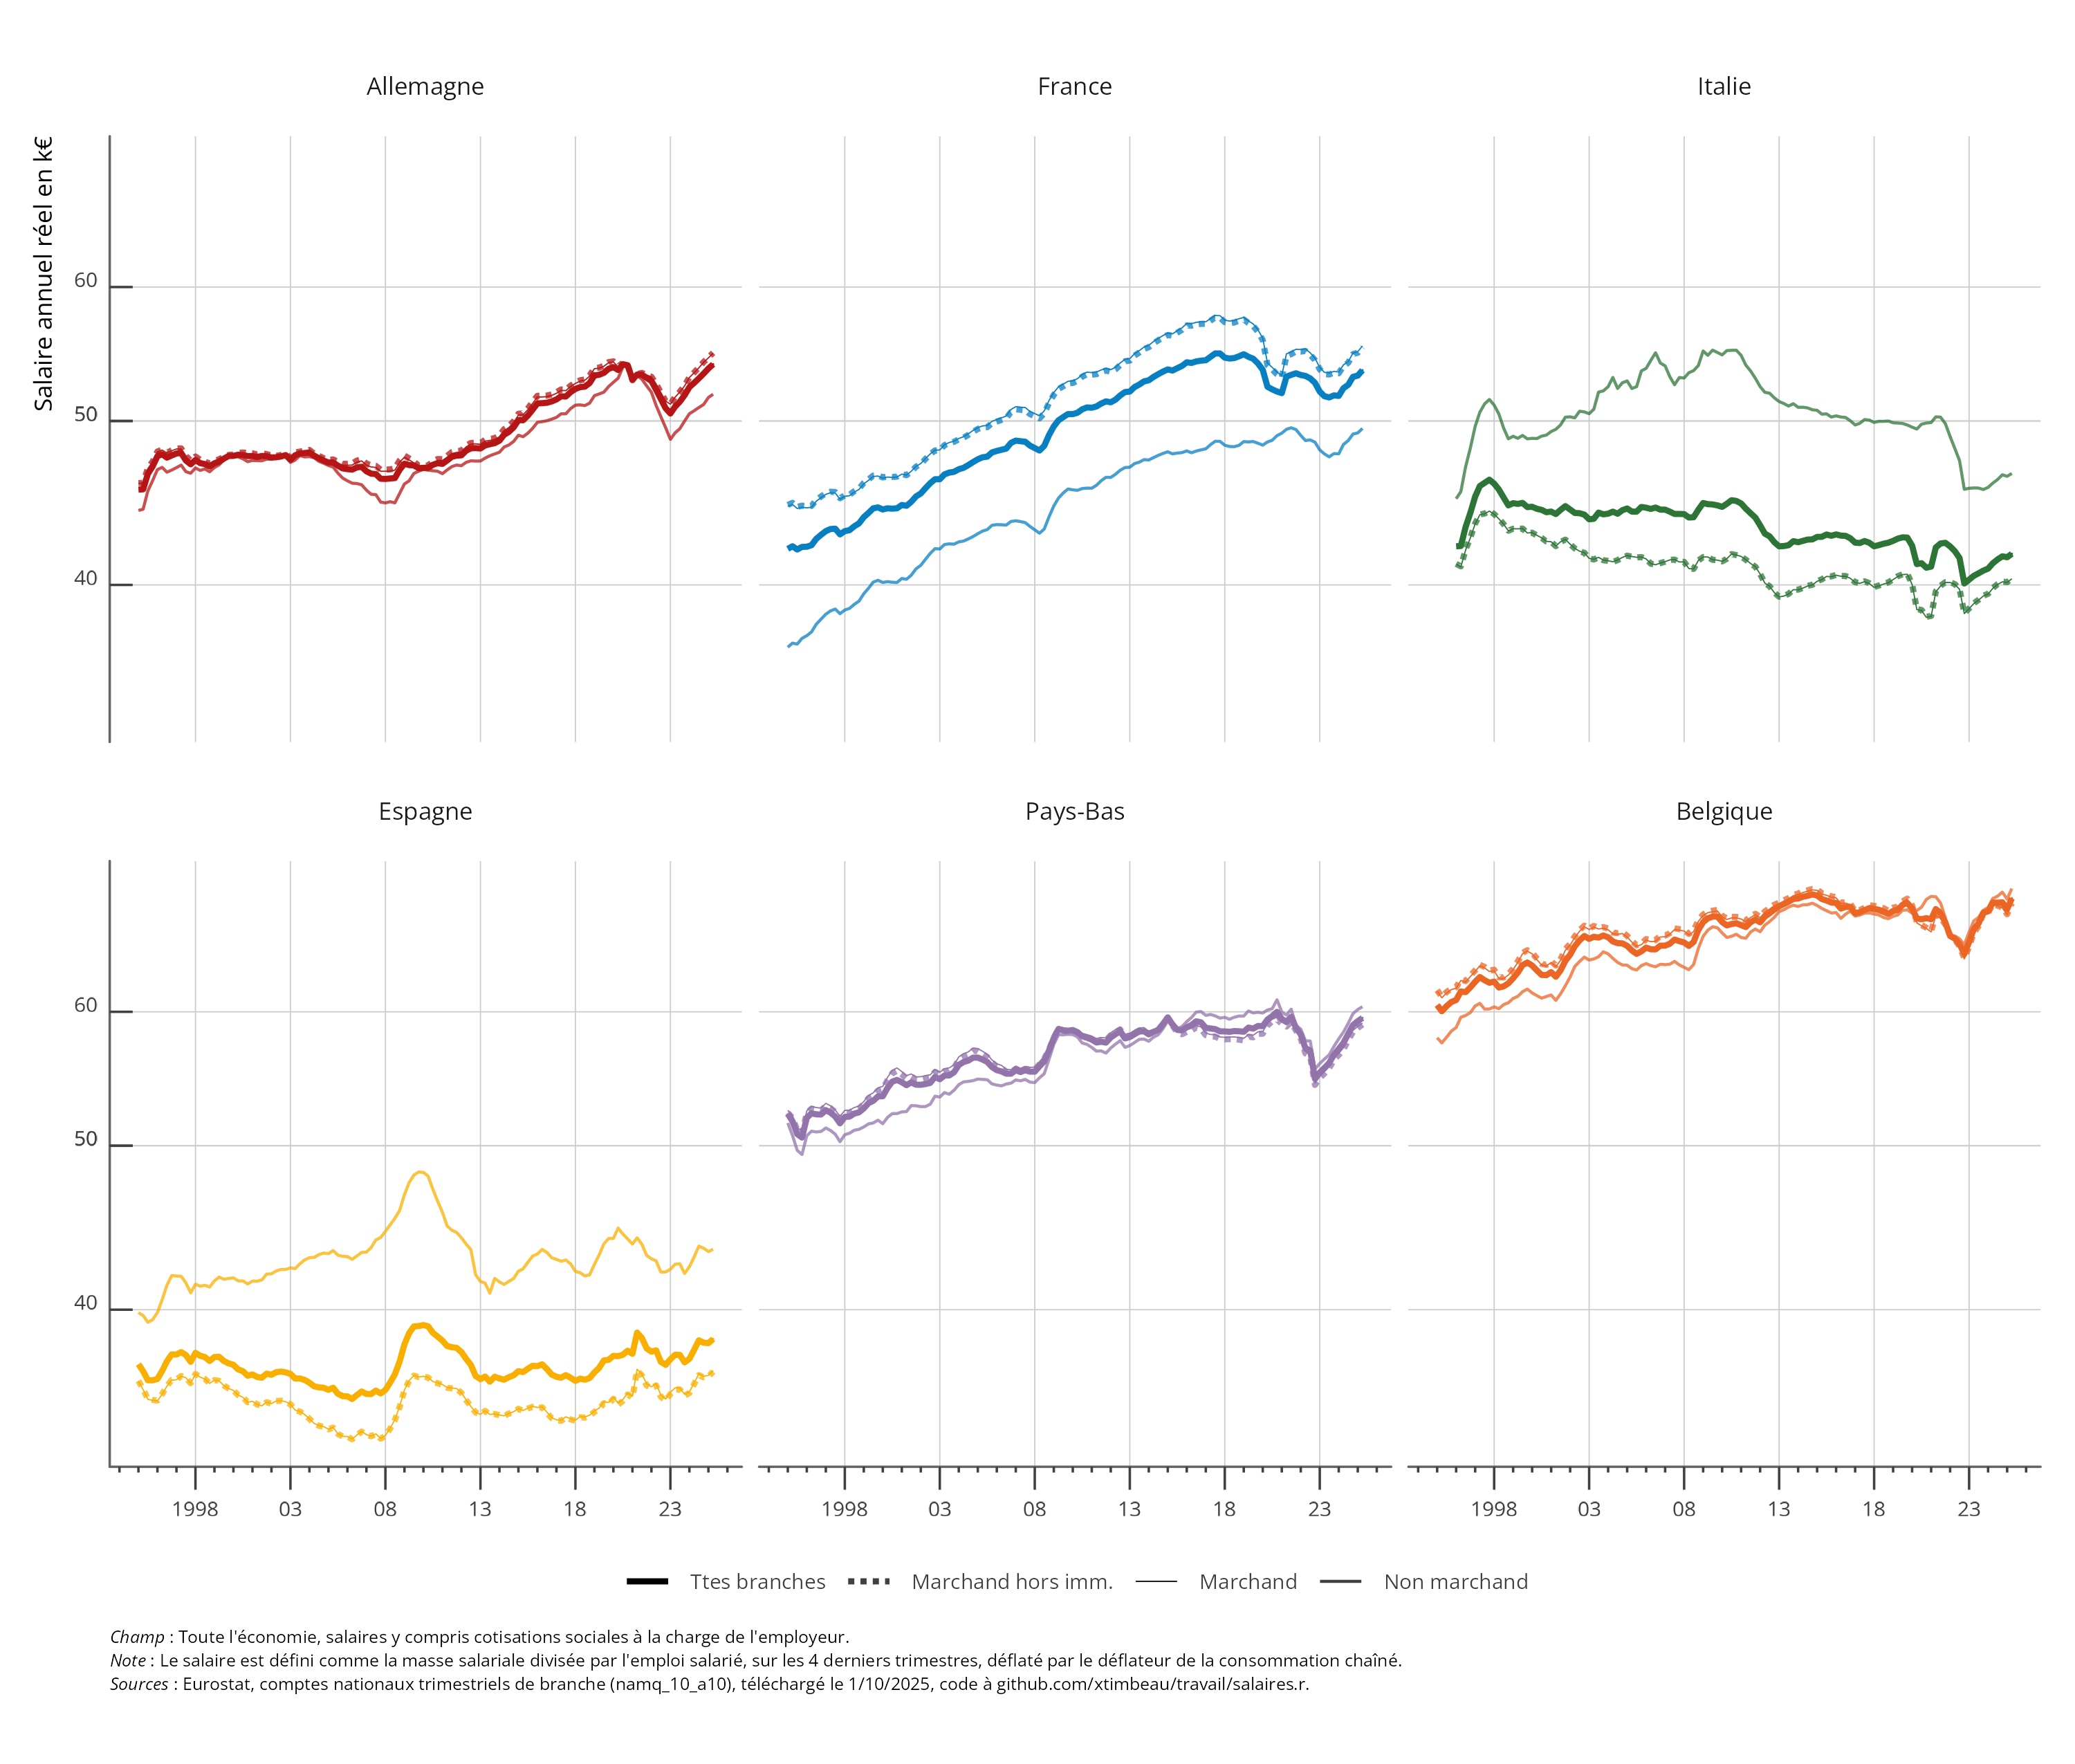
\includegraphics[width=1\linewidth,height=\textheight,keepaspectratio]{psal_comp_files/figure-pdf/fig-salaires-1.png}

}

\end{figure}%

En Italie et en Espagne, la masse salariale dans les branches non
marchandes est supérieures à celle des branches non marchandes. Aux
Pays-Bas et en Allemagne il n'y a pas de différence notable. En France,
elle est significativement plus basse. Notons que les branches non
marchandes ne sont pas nécessairement de l'emploi public et ce dans des
proportions variables suivant les pays. Dans tous les pays, la masse
salariale des branches immobilier et (surtout) services financiers est
plus élevée que la masse salariale dans les autres branches marchandes.

\section{Part des salaires dans la valeur ajoutée, comptes de
branche}\label{part-des-salaires-dans-la-valeur-ajoutuxe9e-comptes-de-branche}

On utilise les données de comptabilité nationale, en trimestriel, par
branche
(\href{https://ec.europa.eu/eurostat/databrowser/view/nasq_10_nf_tr/default/table?lang=en}{\texttt{nasq\_10\_nf\_tr}}),
ré-agrégées au niveau de l'ensemble de l'économie. Le passage par les
comptes de branches permet de distinguer branches marchandes et non
marchandes ou d'autres regroupements, comme l'exclusion des services
immobiliers. Ce passage permet également de conduire la correction
salariés non salariés au niveau des branches. D'après l'INSEE, (voir le
blog
«\,\href{https://blog.insee.fr/combien-pese-l-industrie-en-france-et-en-allemagne/}{Combien
pèse l'industrie en France et en Allemagne}\,»), tous les pays ne
produisent pas une comptabilité de branche mais pour certains (notamment
l'Allemagne) une comptabilité sectorielle. La différence tient aux
entreprises qui produisent plusieurs produits (un constructeur
automobile propose des services financiers pour l'achat des véhicules)
et dont l'activité est imputé à différentes branches (industrie et
services financiers) dans la comptabilité de branche alors que dans une
comptabilité de secteur l'acitvité est versée dans le principal secteur
(ou le secteur d'immatriculation de l'entreprise chapeau). Cette
différence empêche normalement les comparaisons des comptes de branches
entre pays, y compris à l'intérieur de l'Union Européenne. Cependant,
pour comparer la part des salaries dans la valeur ajoutée sur des
agrégats larges (branches marchandes par exemple), cette dérogation à la
norme comptable n'est que modérément problématique\,: de toute façon,
l'automobile et les services financiers sont agrégés et c'est la
correction pour la masse salariale des non salariés qui peut être
modifiée. Mais si la même délimitation est employée pour les salariés et
les non salariés que pour l'activité, l'erreur est probablement minime.

La part des salaires est corrigée de la part des non salariés (données
annuelles
\href{https://ec.europa.eu/eurostat/databrowser/view/nama_10_a64_e/default/table?lang=en}{\texttt{nama\_10\_a64\_e}},
extrapolées en maintenant le ratio salariés/non salariés à sa dernière
valeur observée) en considérant que le salaire des non salariés est
identique dans chaque branche à celui des salariés\,-- cette hypothèse
sous estime probablement le salaire des non salariés mais elle est
difficile à lever, sauf à utiliser les enquêtes force de travail et
faire confiance aux revenus qui y sont déclarés, en perdant la variation
d'une année à l'autre. En revanche, on prend bien en compte que les non
salariés de la branche agricole n'ont pas le même revenu que ceux de la
branche «\,information et communication\,». La décomposition employée
est à 9 branches et on peut conduire la même correction à un niveau de
désagrégation plus fin.

La masse salariale est rapportée soit à la valeur ajoutée brute
(\(B1G\)), soit à la valeur ajoutée nette (\(B1N=B1G-P51C\)). Comme la
consommation de capital fixe (\(P51C\)) n'est pas connue en trimestriel,
elle est dérivée des comptes annuels en 21 branches (niveau 1 de la NACE
rev2 \hyperref[0]{\texttt{nama\_10\_a64}}), agrégée en 9 branches, puis
extrapolée pour les années non connues (ici 2024 et 2025) en conservant
un ratio constant dans la valeur ajouté brute. Le détail se trouve dans
le code.

Les trois graphiques suivants illustrent les conséquences sur la mesure
de la part des salaires suivant les différents concepts. Le
graphique~\ref{fig-psalcnc} compare avec et sans correction pour les non
salariés. Deux rubans sont affichés, l'un pour les branches marchandes
hors services immobiliers et financiers et l'autre pour toutes les
branches.

L'avantage des comptes de branches est une définition homogène pour
chacun des pays. La branche immobilier est exclue parce qu'il est
impossible de distinguer les entreprises des ménages propriétaires (les
loyers imputés sont une valeur ajoutée des ménages).

Les données trimestrielles sont annualisées pour la lisibilité et pour
simplifier le mélange de données annuelles et trimestrielles. Le point
2025 (la dernière année) est donc un acquis sur les trimestres observés
de l'année (ici 2 trimestres sur 4) suceptible de changer au fur et à
mesure du temps. Il est possible en modifiant le code de produire un
graphique trimestriel ou trimestriel lissé, à votre convenance.

\begin{figure}[H]

\caption{\label{fig-psalcnc}Correction pour la non salarisation ou non,
comptes de branches}

\centering{

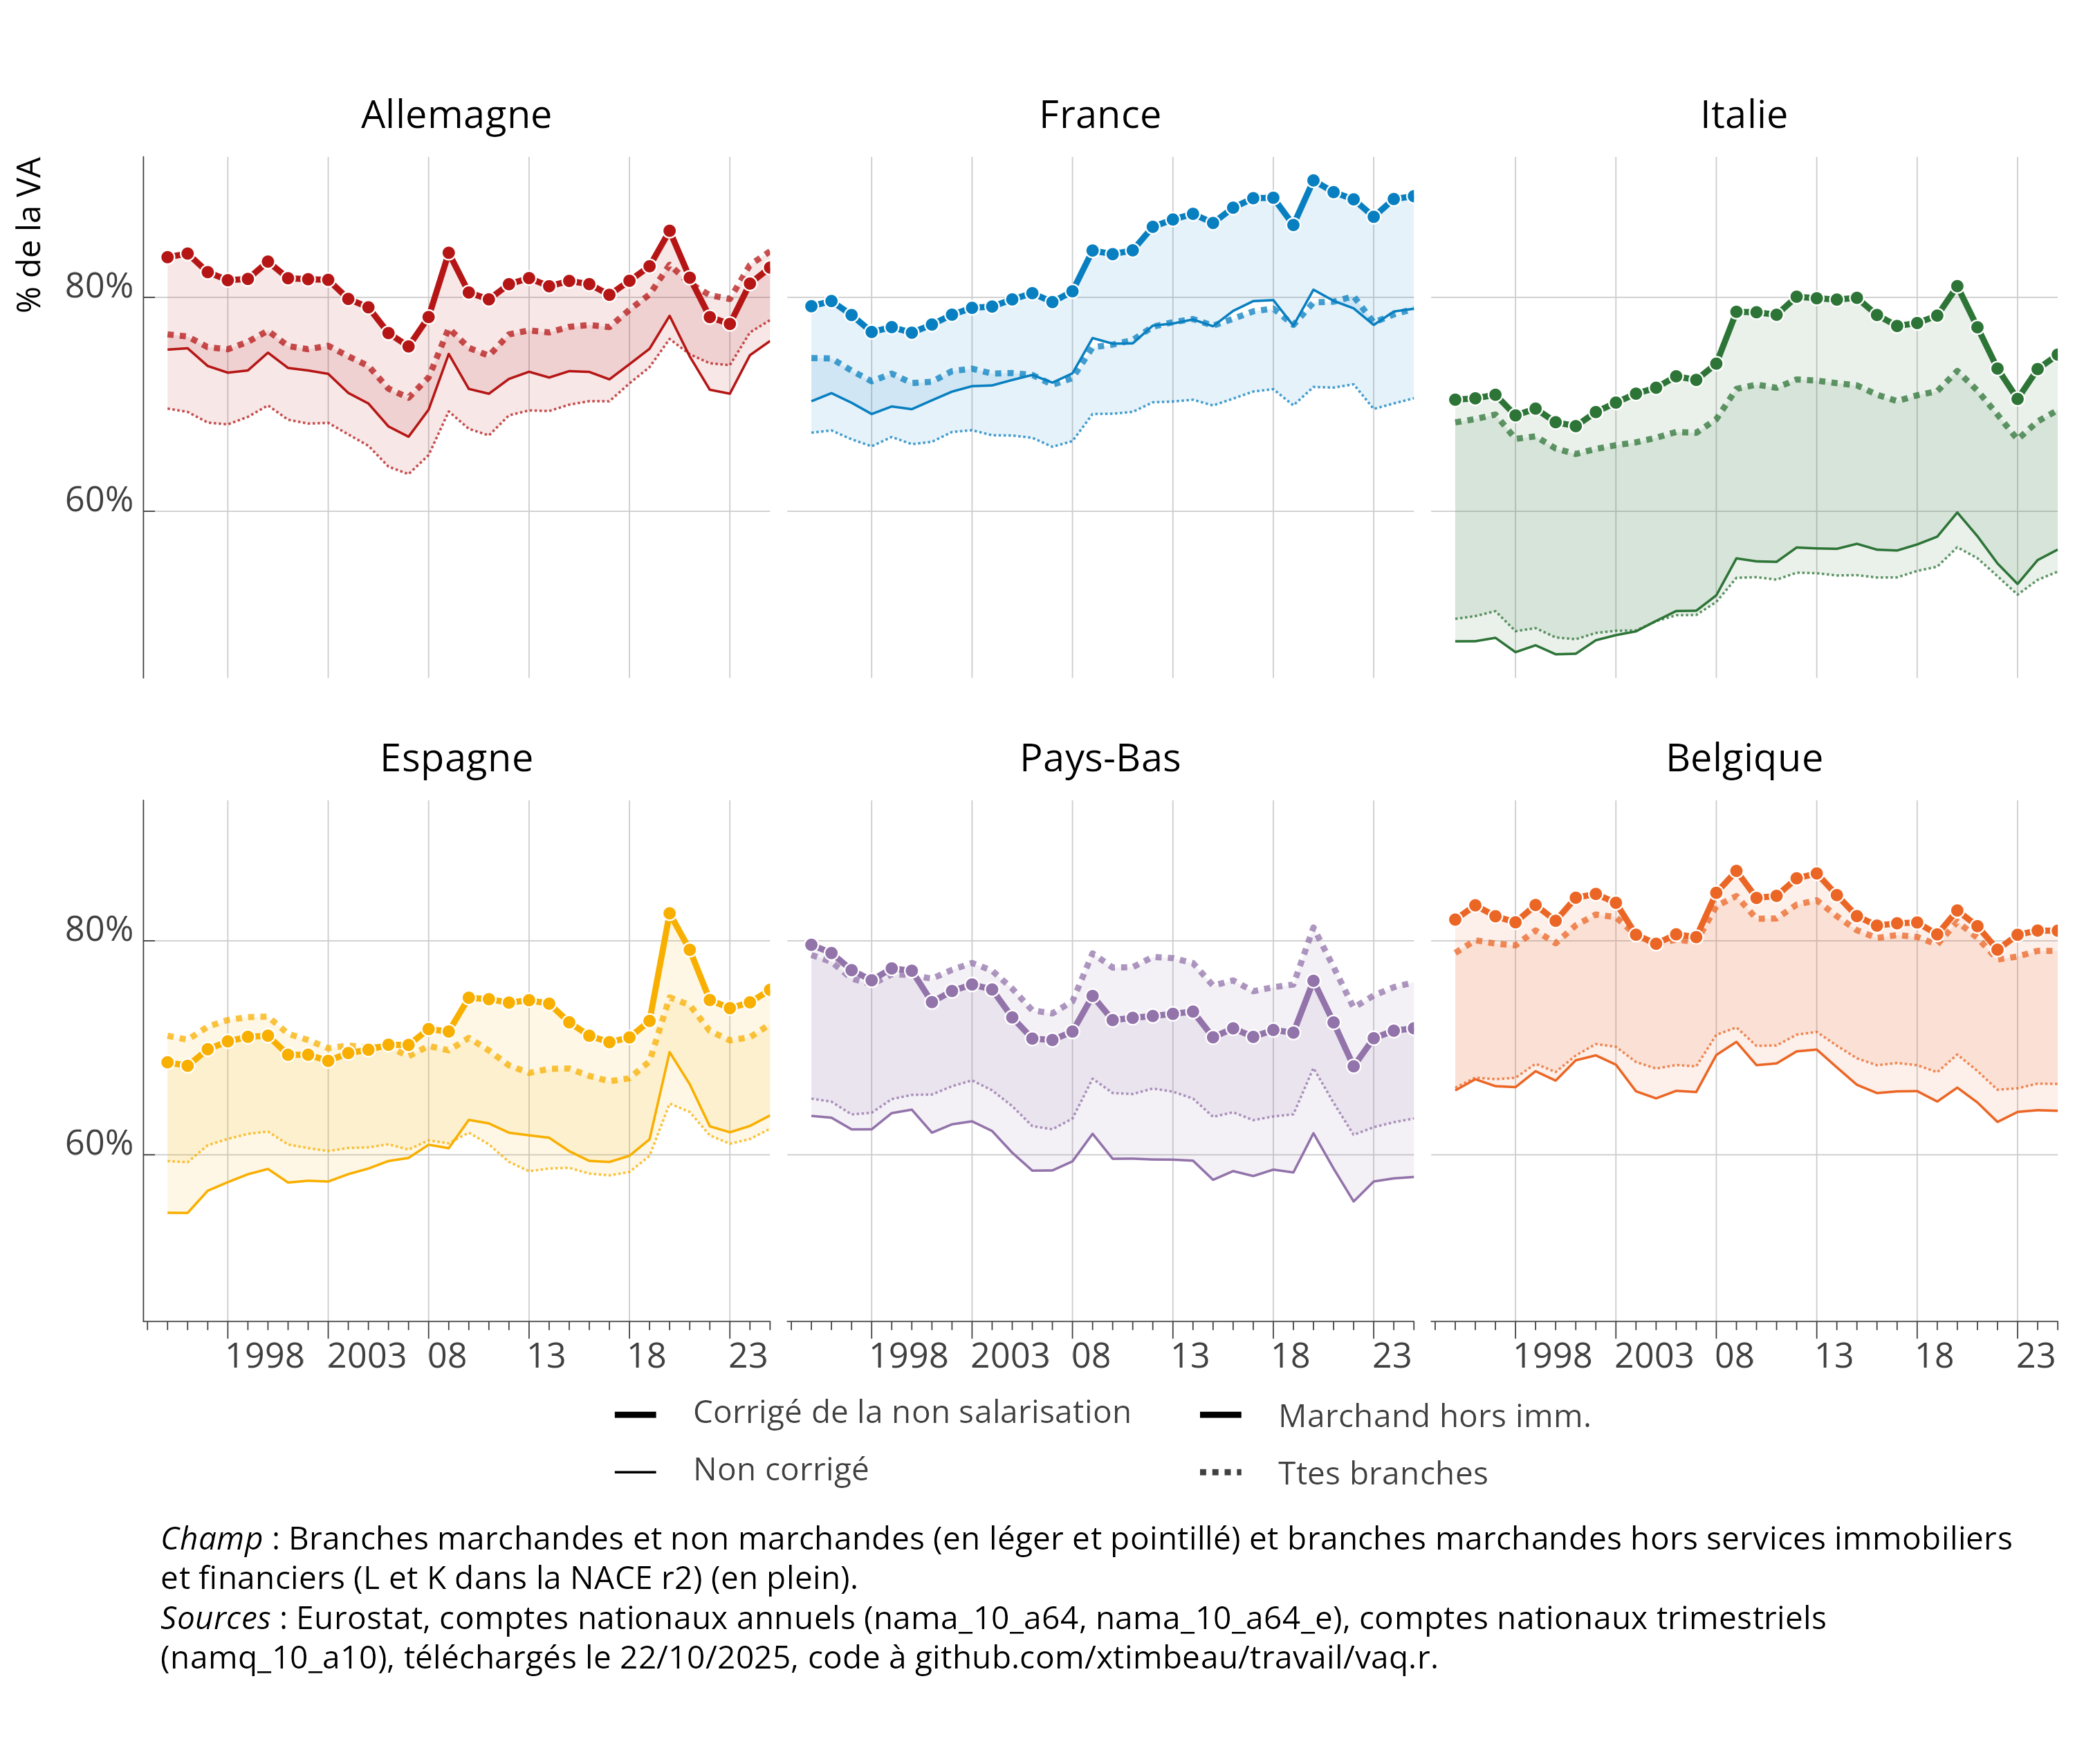
\includegraphics[width=1\linewidth,height=\textheight,keepaspectratio]{psal_comp_files/figure-pdf/fig-psalcnc-1.png}

}

\end{figure}%

La correction de la non salarisation, en imputant une masse salariale
pour les entrepreneurs individuels, augmente la part des salaires. La
correction n'est pas constante dans le temps (c'est particulièrement
fort pour la France) ni dans l'espace (la correction est très forte en
Italie). La correction est plus importante lorsqu'on se limite aux
branches marchandes hors services immobiliers et services financiers,
sauf aux Pays-Bas.

\begin{figure}[H]

\caption{\label{fig-psalnetbrut}Nette ou brute, comptes de branches}

\centering{

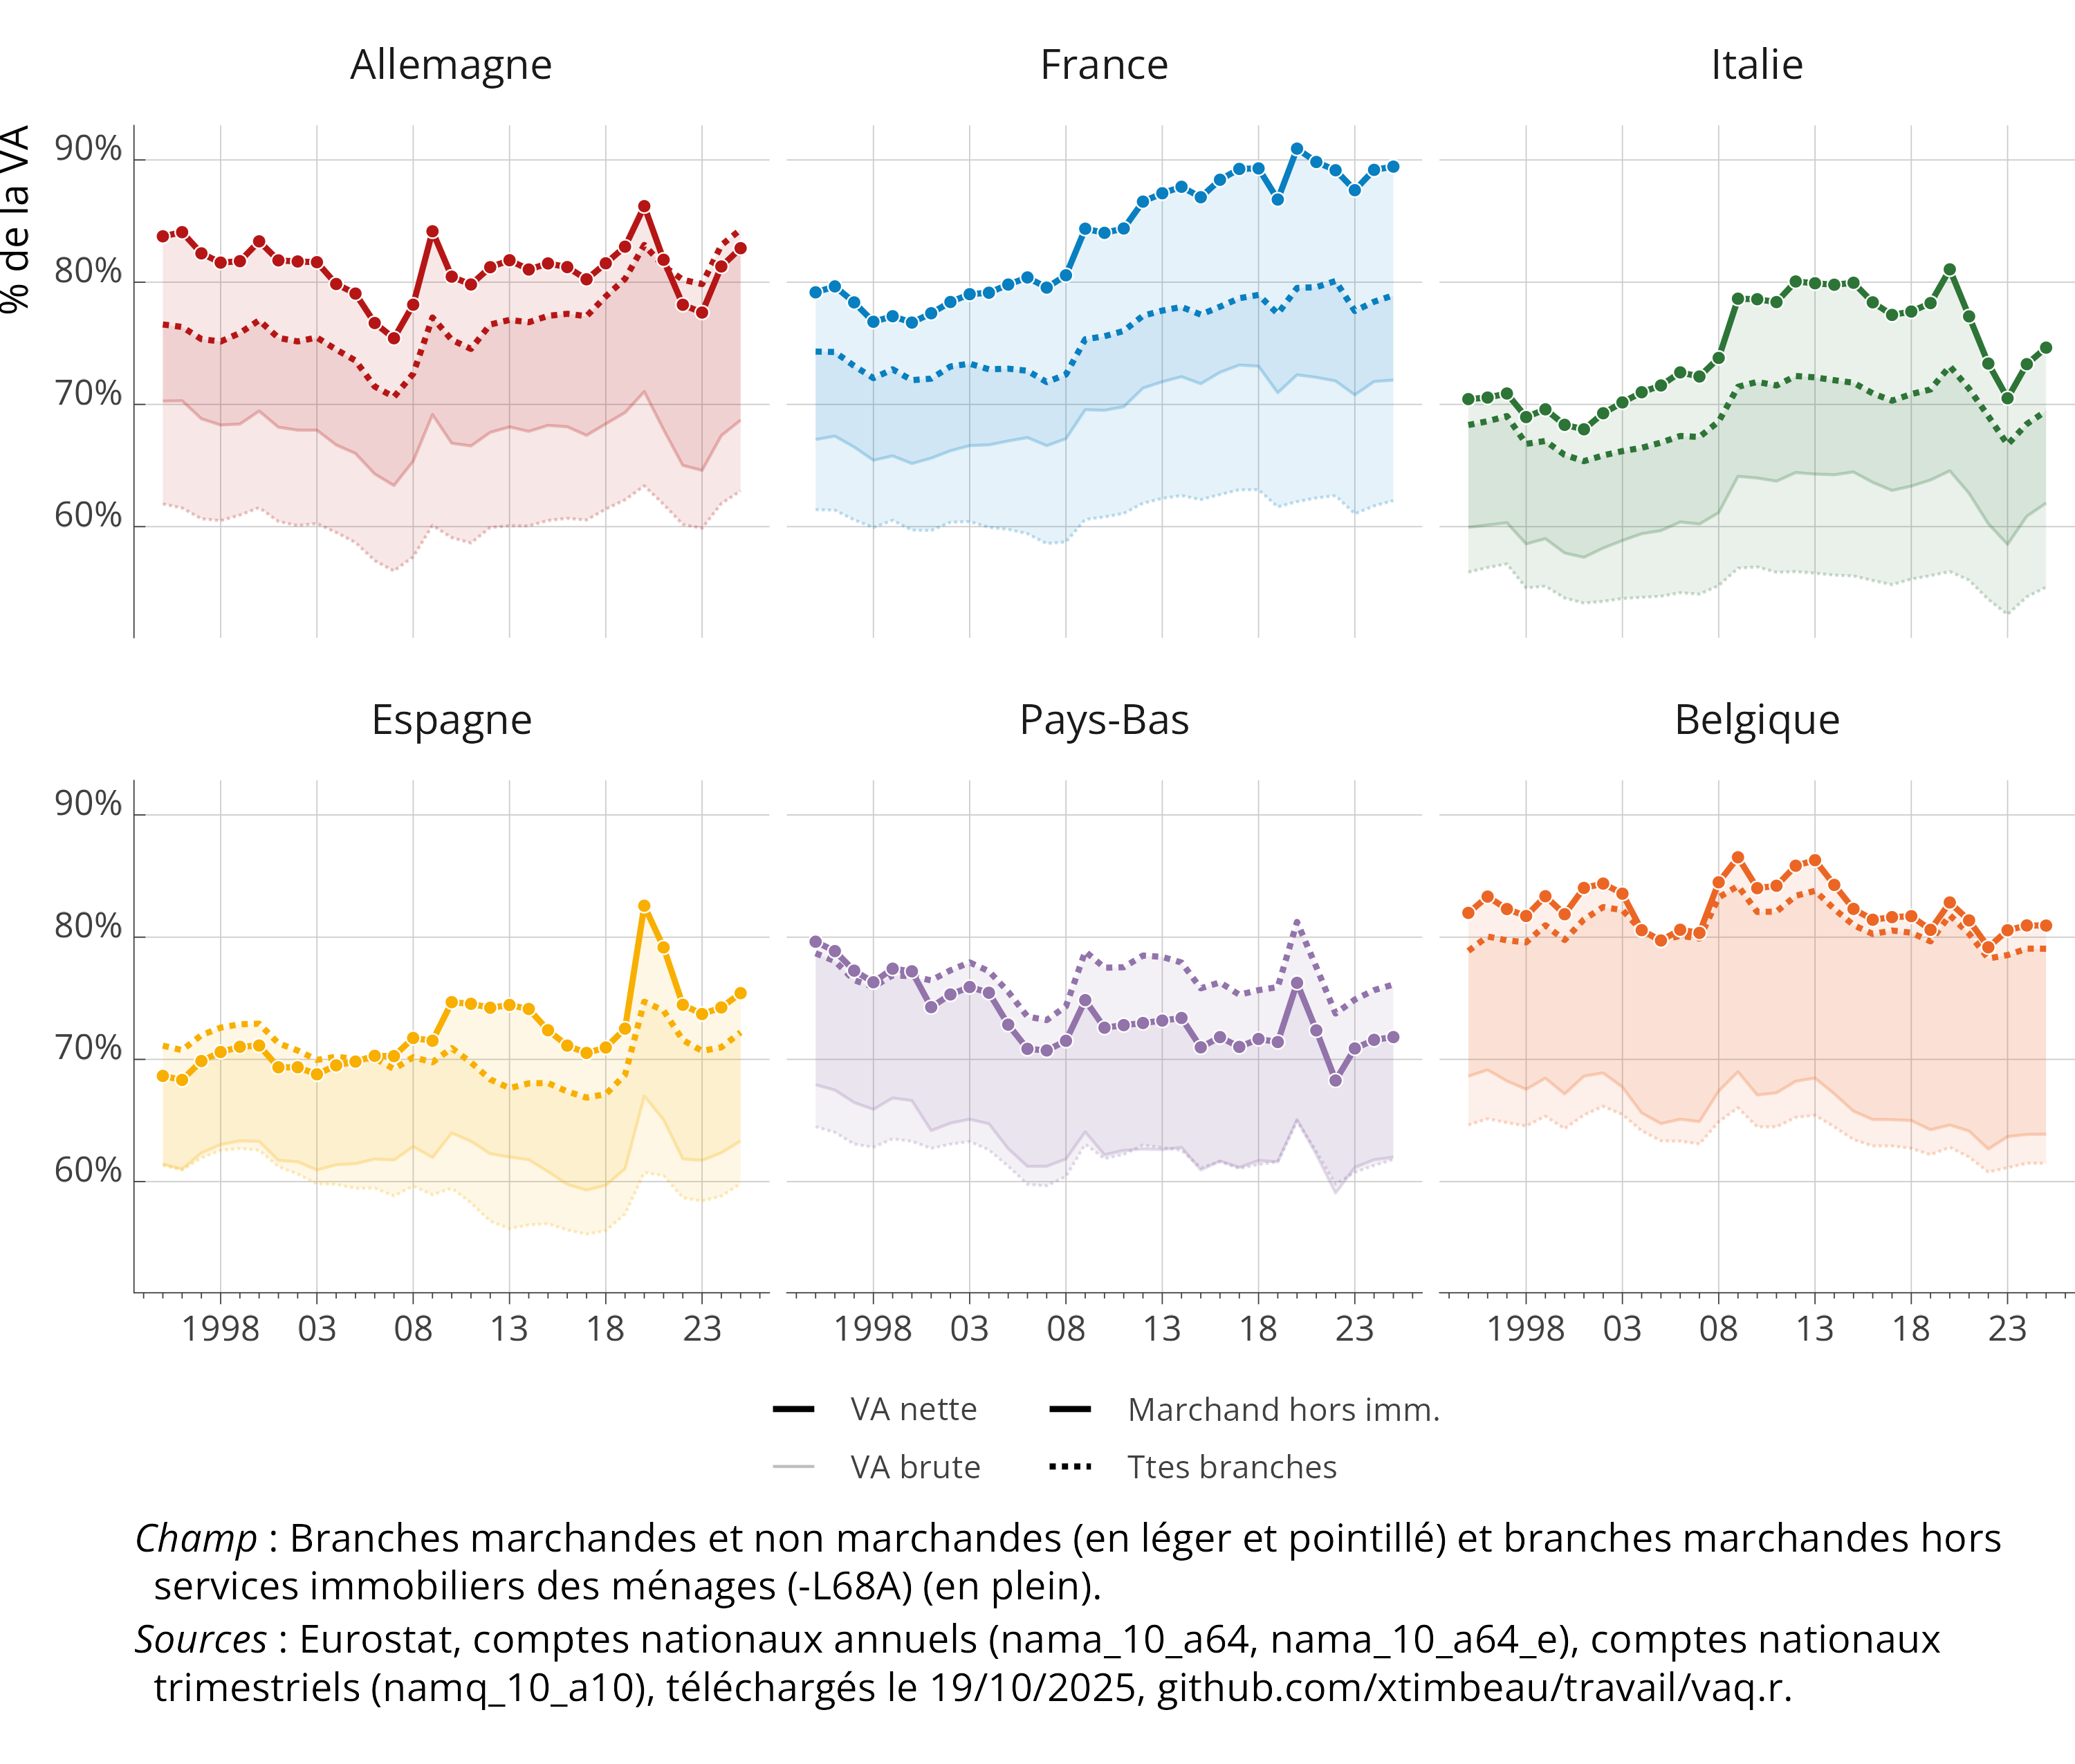
\includegraphics[width=1\linewidth,height=\textheight,keepaspectratio]{psal_comp_files/figure-pdf/fig-psalnetbrut-1.png}

}

\end{figure}%

La notion de part des salaires dans la valeur ajoutée nette consiste à
réduire le démominateur (la valeur ajoutée) de la consommation de
capital fixe. Cela augmente donc le ratio. Cependant, cette correction
n'est pas constante dans le temps (comme en France, en Espagne ou en
Belgique). Comme on peut le voir sur le graphique~\ref{fig-psalcompote},
la variance entre les pays est plus basse pour la notion brute (non
corrigé de la CCF) que nette. Pour les branches marchandes hors services
immobiliers et services immobiliers, le classement entre pays est
marginalement modifié, la Belgique ayant une part des salaires nette pus
élevée que l'Allemagne, alors que sa part brute est plus faible qu'en
Allemagne. Pour les autres pays, le classement est indentique (La France
a la part la plus haute et les Pays-Bas plus faible).

\begin{figure}[H]

\caption{\label{fig-psalcompote}Tous concepts, comparaison entre pays}

\centering{

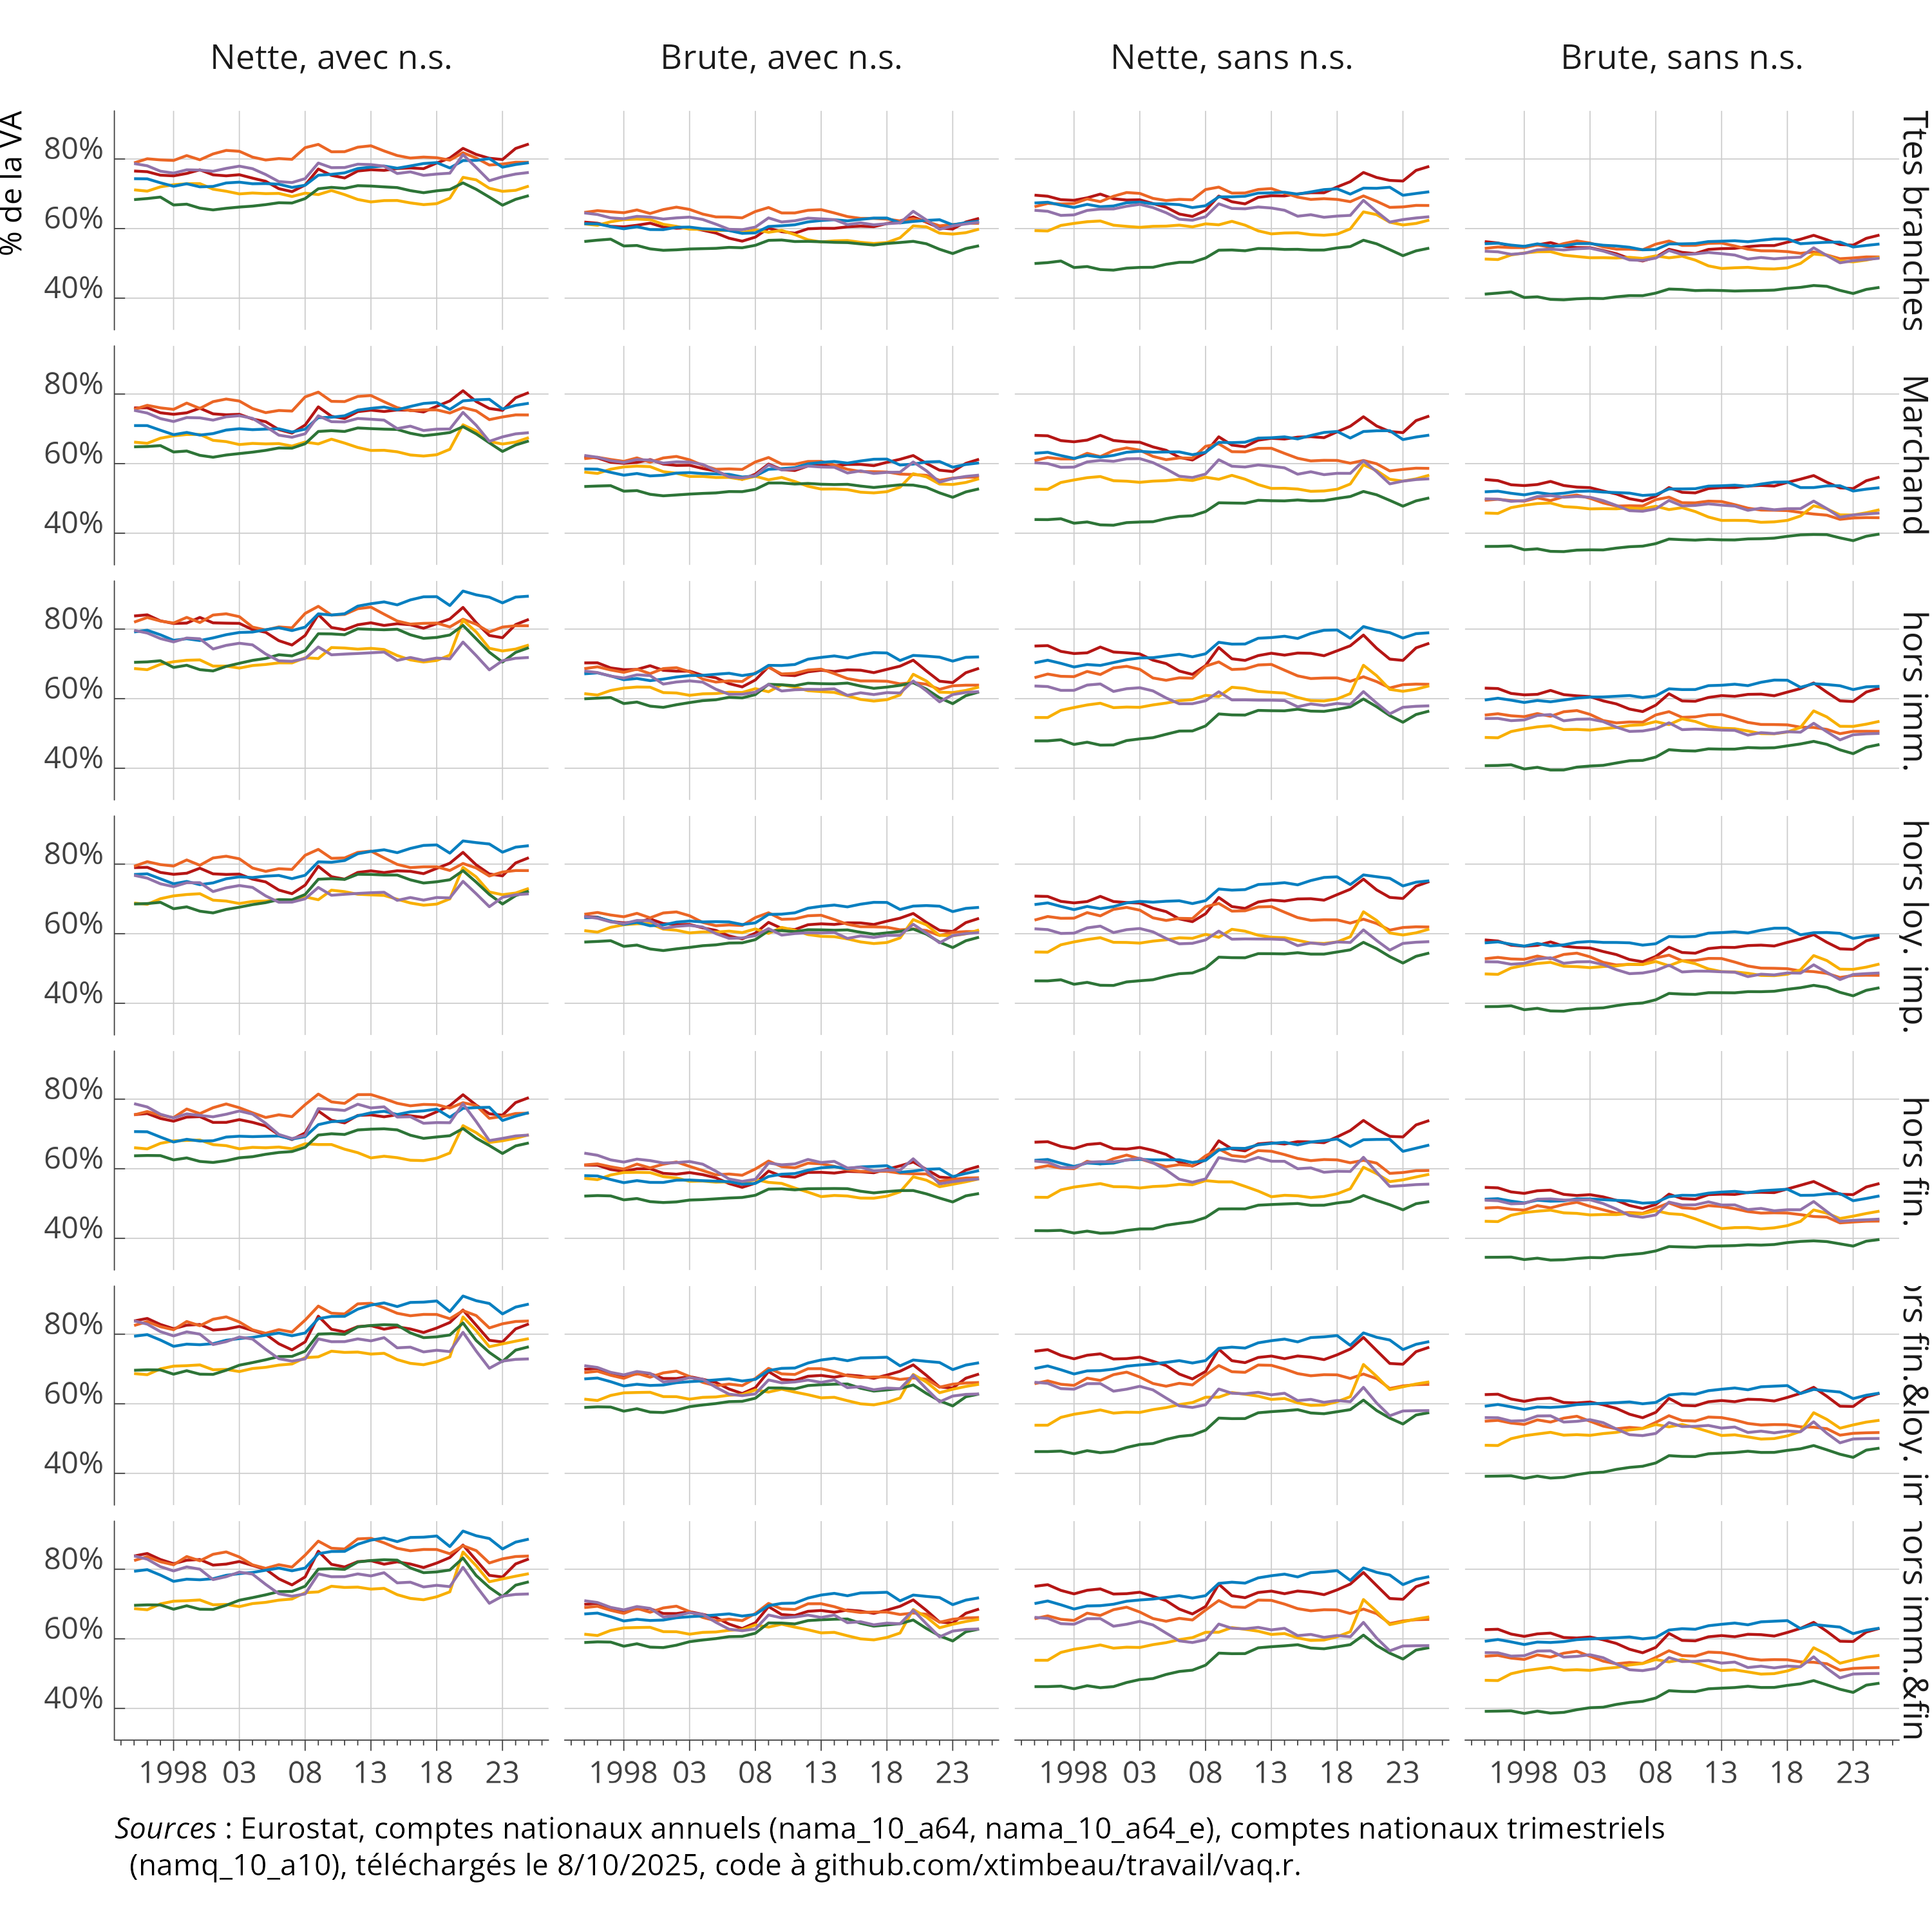
\includegraphics[width=1\linewidth,height=\textheight,keepaspectratio]{psal_comp_files/figure-pdf/fig-psalcompote-1.png}

}

\end{figure}%

\section{Impact du changement de structure de
l'économie}\label{impact-du-changement-de-structure-de-luxe9conomie}

On peut décomposer le changement de la part des salaires dans la valeur
ajoutée en un effet de structure en branche et un effet de changement de
la part des salaires dans la valeur ajoutée dans chaque branche.
Formellement la décomposition retenue s'écrit (où \(w_{b,t}\) est la
part de VAN de la branche \(b\) dans la valeur ajoutée nette de
l'ensemble des branches considérées et \(s_{b,t}\) la part des salaires
dans la branche \(b\))\,:

\[
s_t - \sum w_{b,1995} \times s_{b,1995} =  \sum w_{b,1995} \times (s_{b,t}-s_{b,1995}) + \sum (w_{b,t} - w_{b,1995}) \times s_{b,t}  
\]

L'année 1995 est l'année de référence et le premier terme (de droite)
s'interprète comme la part des salaires qui prévaudrait s'il n'y avait
pas eu de changement de structure. Le \textbf{?@fig-structbanche}
représente ce terme ainsi que la part agrégée des salaires (\(s_{t}\)).
Leffet de la structure par branche de l'économie (ici marchande hors
services immobiliers produits par les ménages) est assez marginale. Les
variations de la part des salaires sont bien celle des parts des
salaires dans chaque secteur.

Il existe quelques exceptions à cette régle générale. A structure de
branche inchangée, avec comme année de référence 1995, la part des
salaires serait plus basse de 3,5~points de VA pour les Pays-Bas en
2025. En Allemagne ou en Belgique, le changement de structure des
branches explique un petit peu de l'évolution à la hausse.

En revanche, la part des salaires serait légèrement supérieure en Italie
à structure inchangée. Le pic de valeur ajoutée en 2013 est lié
entièrement à la structure par branche, ce qui laisse supposer une
rupture de série dans les comptes de branche.

\begin{figure}[H]

\caption{\label{fig-structbranche}Structure par branche et part des
salaires dans la VA}

\centering{

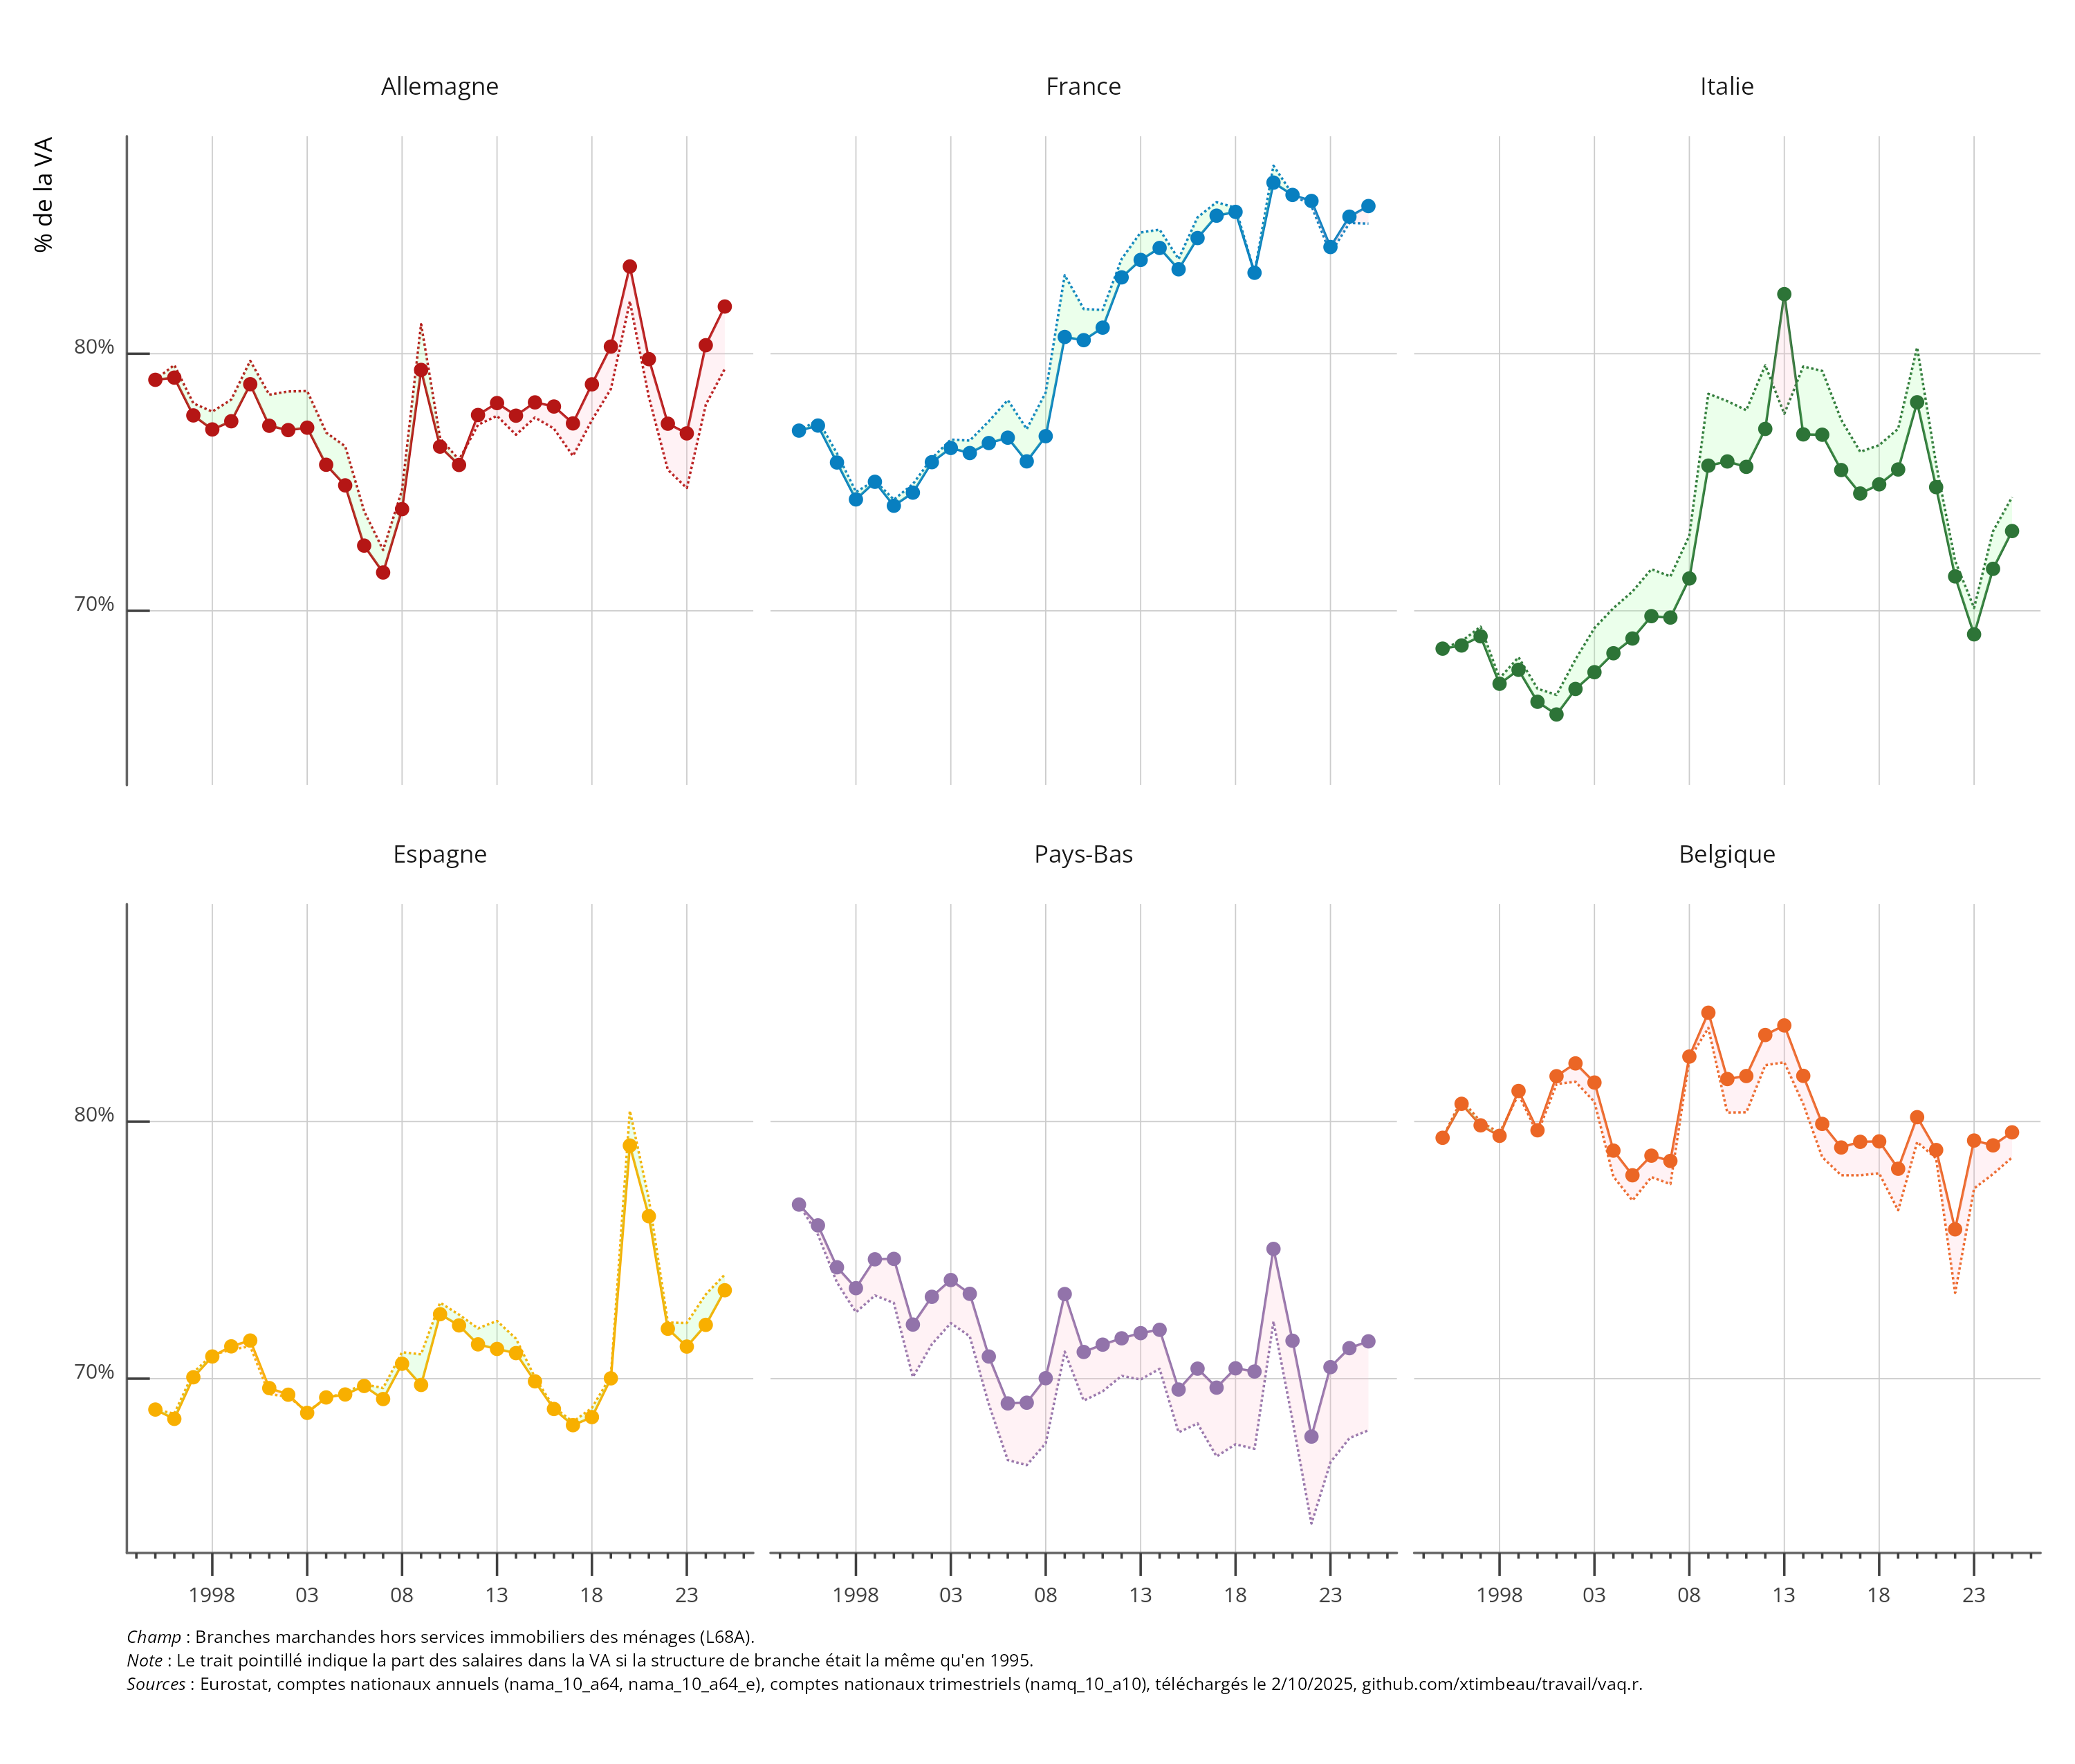
\includegraphics[width=1\linewidth,height=\textheight,keepaspectratio]{psal_comp_files/figure-pdf/fig-structbranche-1.png}

}

\end{figure}%

\section{Part des salaires dans la valeur ajoutée, comptes
d'agents}\label{part-des-salaires-dans-la-valeur-ajoutuxe9e-comptes-dagents}

Les comptes d'agents (ou de secteurs institutionnels) permettent une
analyse plus simple, parce qu'ils permettent de distinguer les seules
entreprises non financières. Cela évite d'avoir à prendre en compte les
non salariés, cela exclue les services immobiliers produits par les
ménages. C'est donc une analyse sur un champ économique plus strict (au
sens de la forme légale des entités considérées). La notion d'impôt sur
les sociétés est aussi mieux définie et le stock de capital productif
est mieux connu du fait de l'obligation légale de déclaration des
comptes des entreprises.

Malheureusement, comme identifié par l'INSEE, la pratique des instituts
nationaux européens n'est pas conforme à celle de l'INSEE. Par exemple,
en Allemagne, le secteur S11 inclut les quasi-sociétés et les
entrepreneurs individuels. La normalisation des concepts est par
ailleurs peu probable dans le futur, puisqu'elle est liée aux pratiques
administratives.

Comme pour les graphiques précédents, les données trimestrielles sont
annualisées (pour éliminer la variabilité trimestrielle qui nuit à la
lisibilité et qui n'a pas beaucoup de sens). En trait pointillé, on
représente la part de la valeur ajoutée dans les branches marchandes
hors immobilier et corrigée de la non salarisation pour mesurer la
différence des concepts.

\begin{figure}[H]

\caption{\label{fig-s11psal}Part des salaires dans la VA, SNF, comptes
d'agents}

\centering{

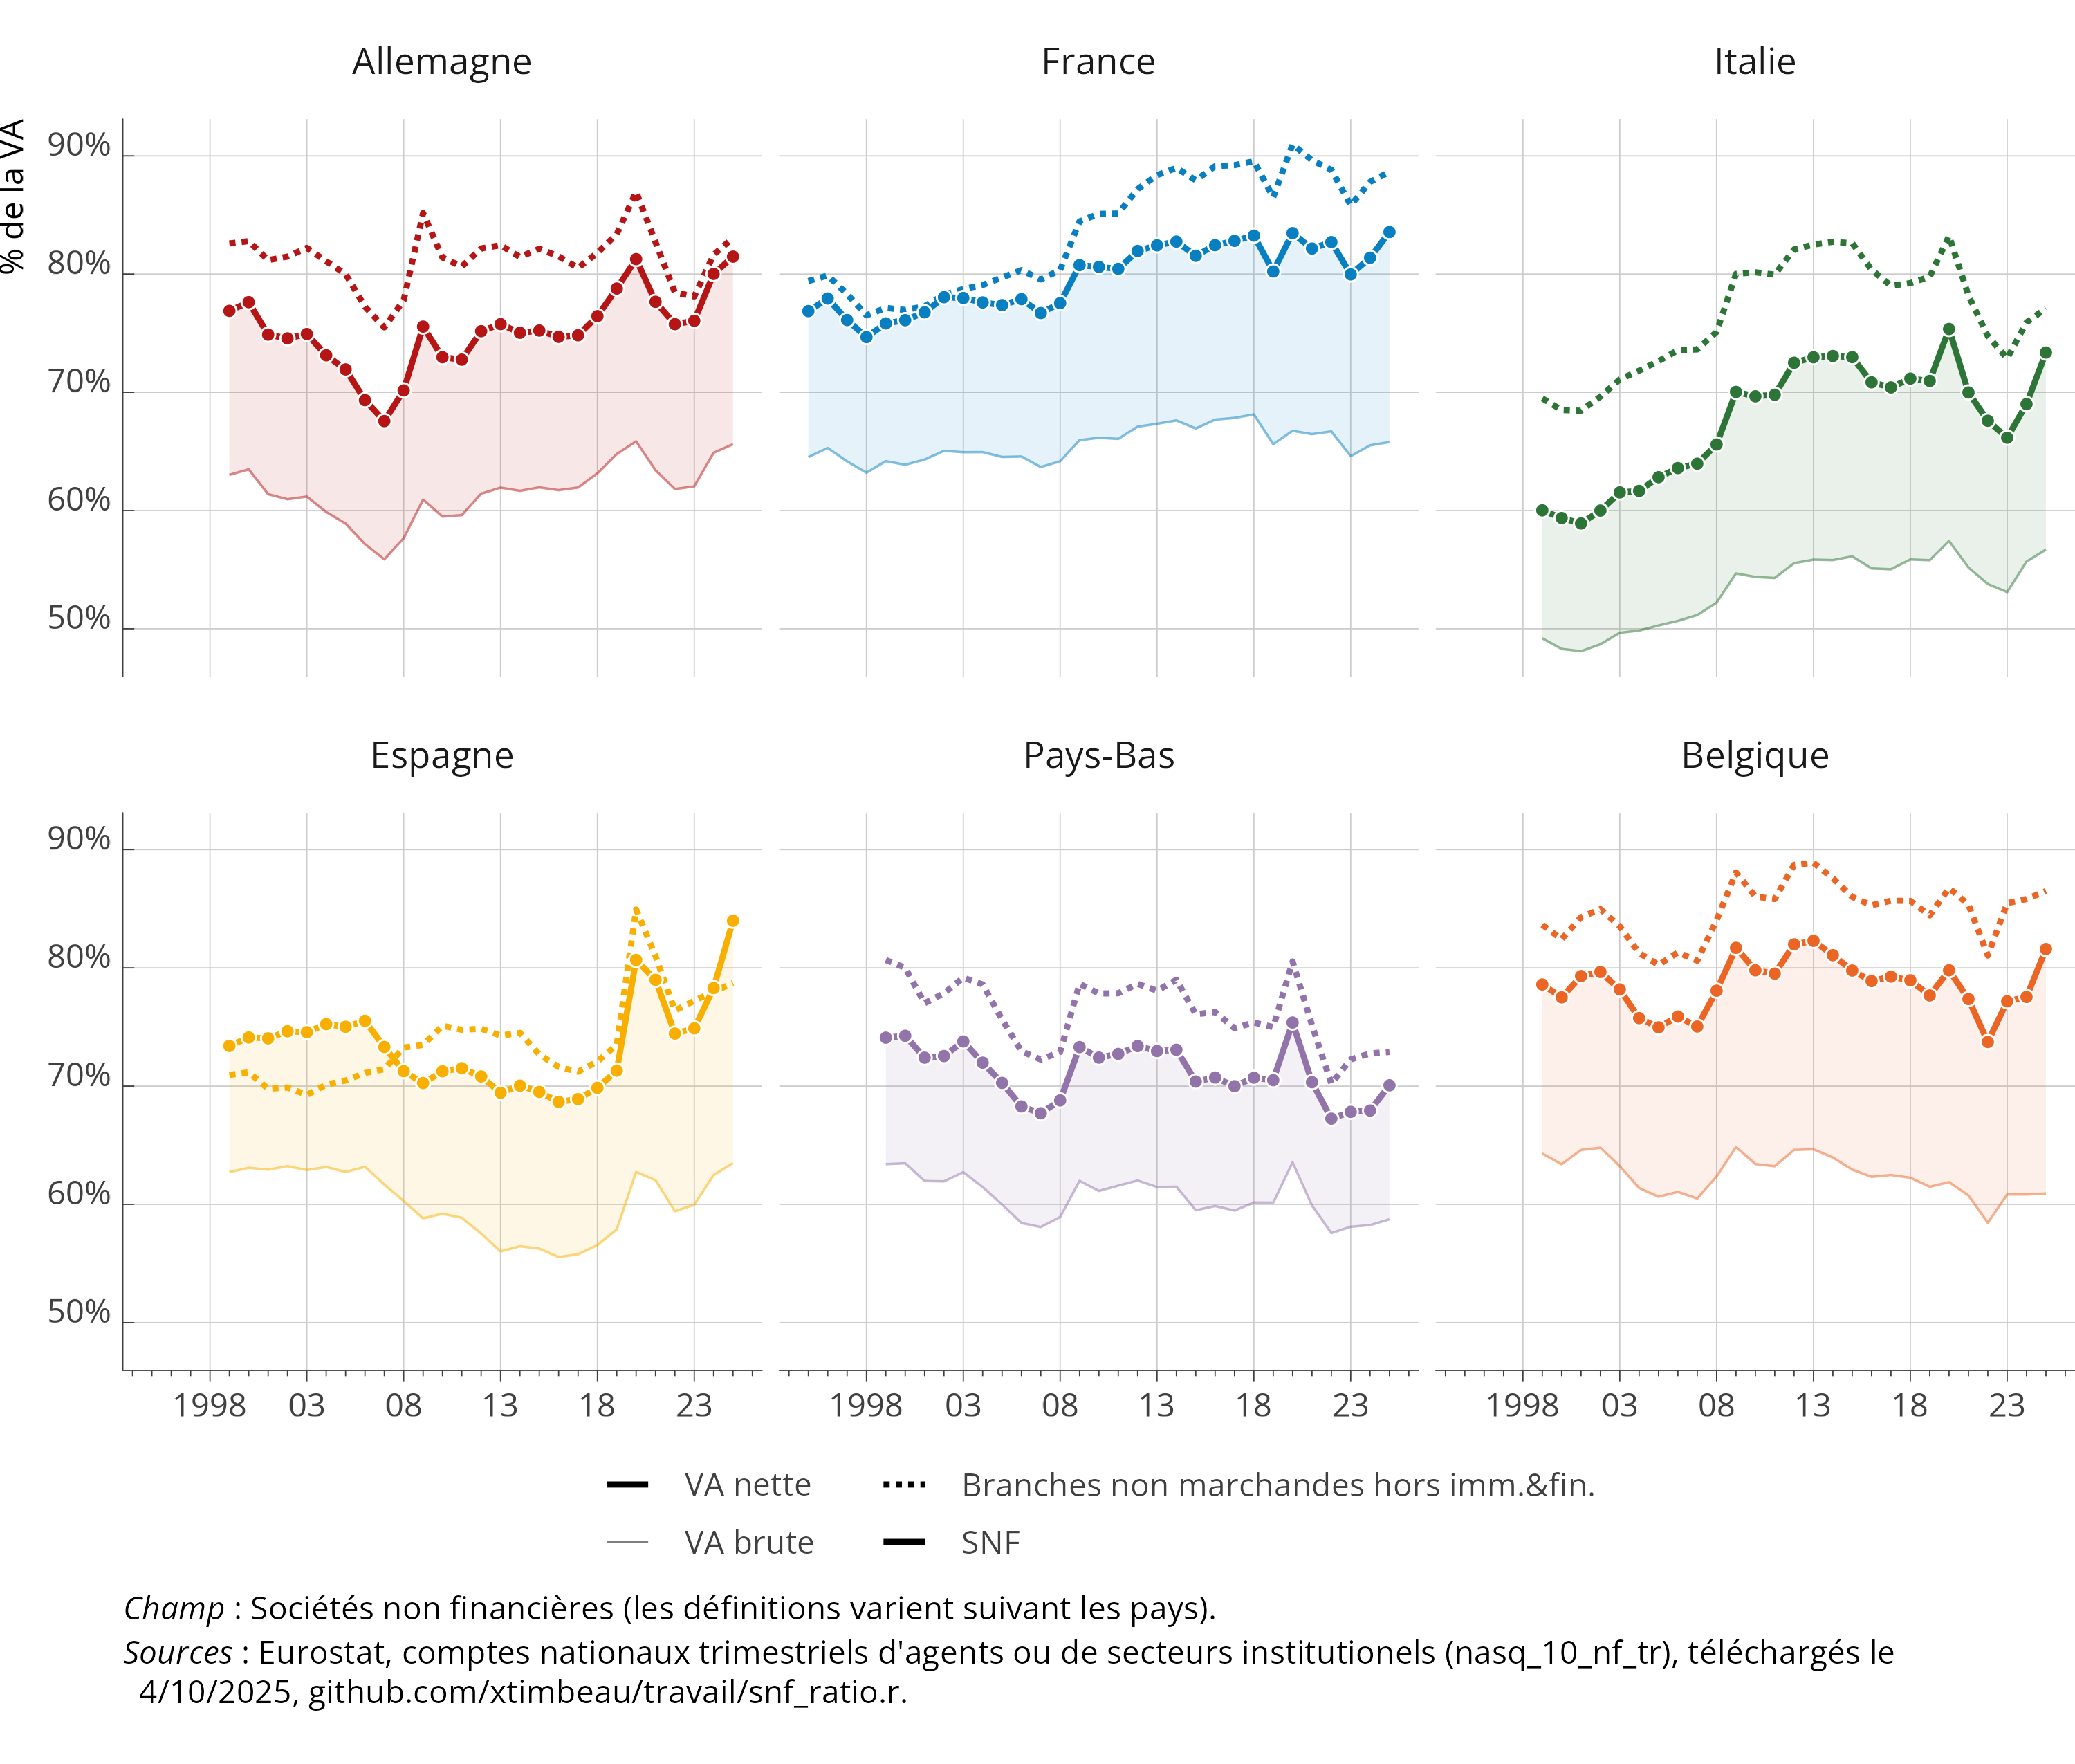
\includegraphics[width=1\linewidth,height=\textheight,keepaspectratio]{psal_comp_files/figure-pdf/fig-s11psal-1.png}

}

\end{figure}%

\begin{figure}[H]

\caption{\label{fig-s1112psal}Part des salaires dans la VA, SNF+SF,
comptes d'agents}

\centering{

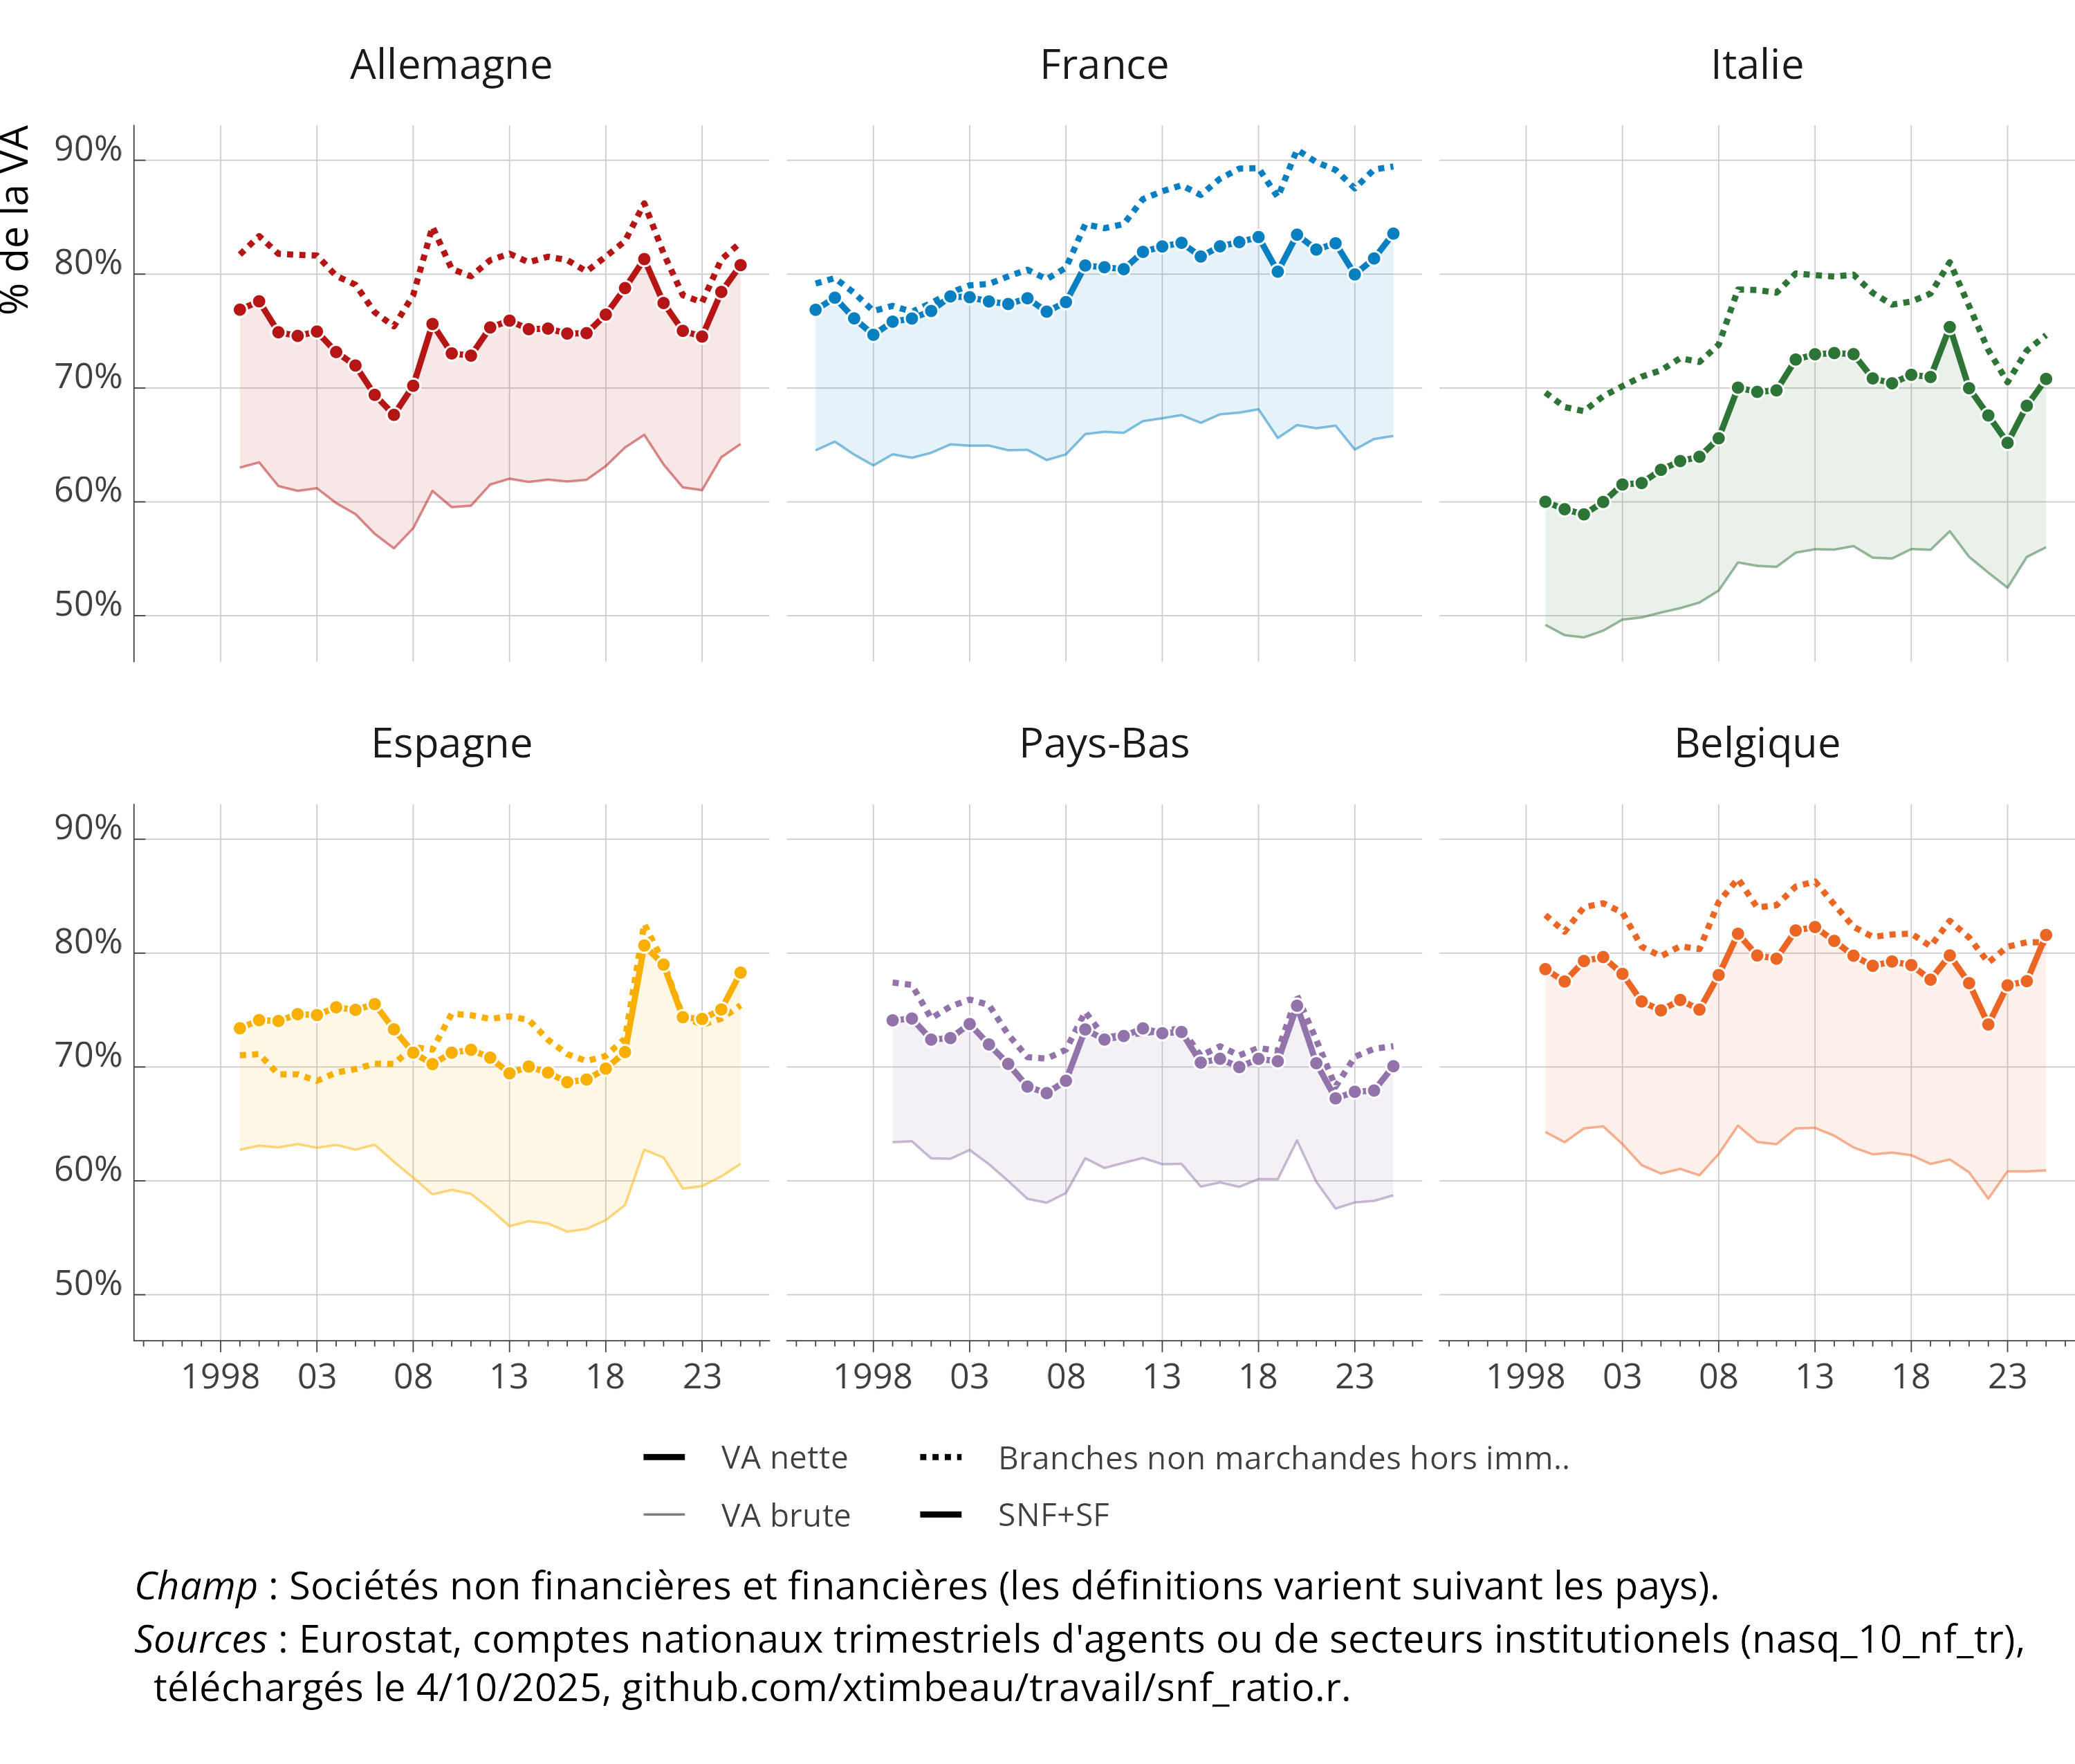
\includegraphics[width=1\linewidth,height=\textheight,keepaspectratio]{psal_comp_files/figure-pdf/fig-s1112psal-1.png}

}

\end{figure}%

\section{Profits nets et dividendes dans les comptes
d'agents}\label{profits-nets-et-dividendes-dans-les-comptes-dagents}

Les comptes des sociétés non financières permettent d'examiner d'autres
éléments du compte. On affiche ici le profit net sur la valeur ajoutée
nette, et le taux de dividendes nets sur la valeur ajoutée nette.

Les profits nets sont définis comme la valeur ajoutée nette de la
consommation de capital fixe moins la rémunération des salariés, moins
les taxes nettes des subventions moins l'impôt sur les sociétés\,:

\[
\Pi = B1G - P51C - D1 - (D2-D3) - D5 = B2N-D5
\]

Les dividendes sont la ligne \(D42\) nette de ce qui est payé et reçu
par le secteur des sociétés non financières (SNF ou S11).

\begin{figure}[H]

\caption{\label{fig-profits}Profits nets dans la VA, SNF, comptes de
secteur}

\centering{

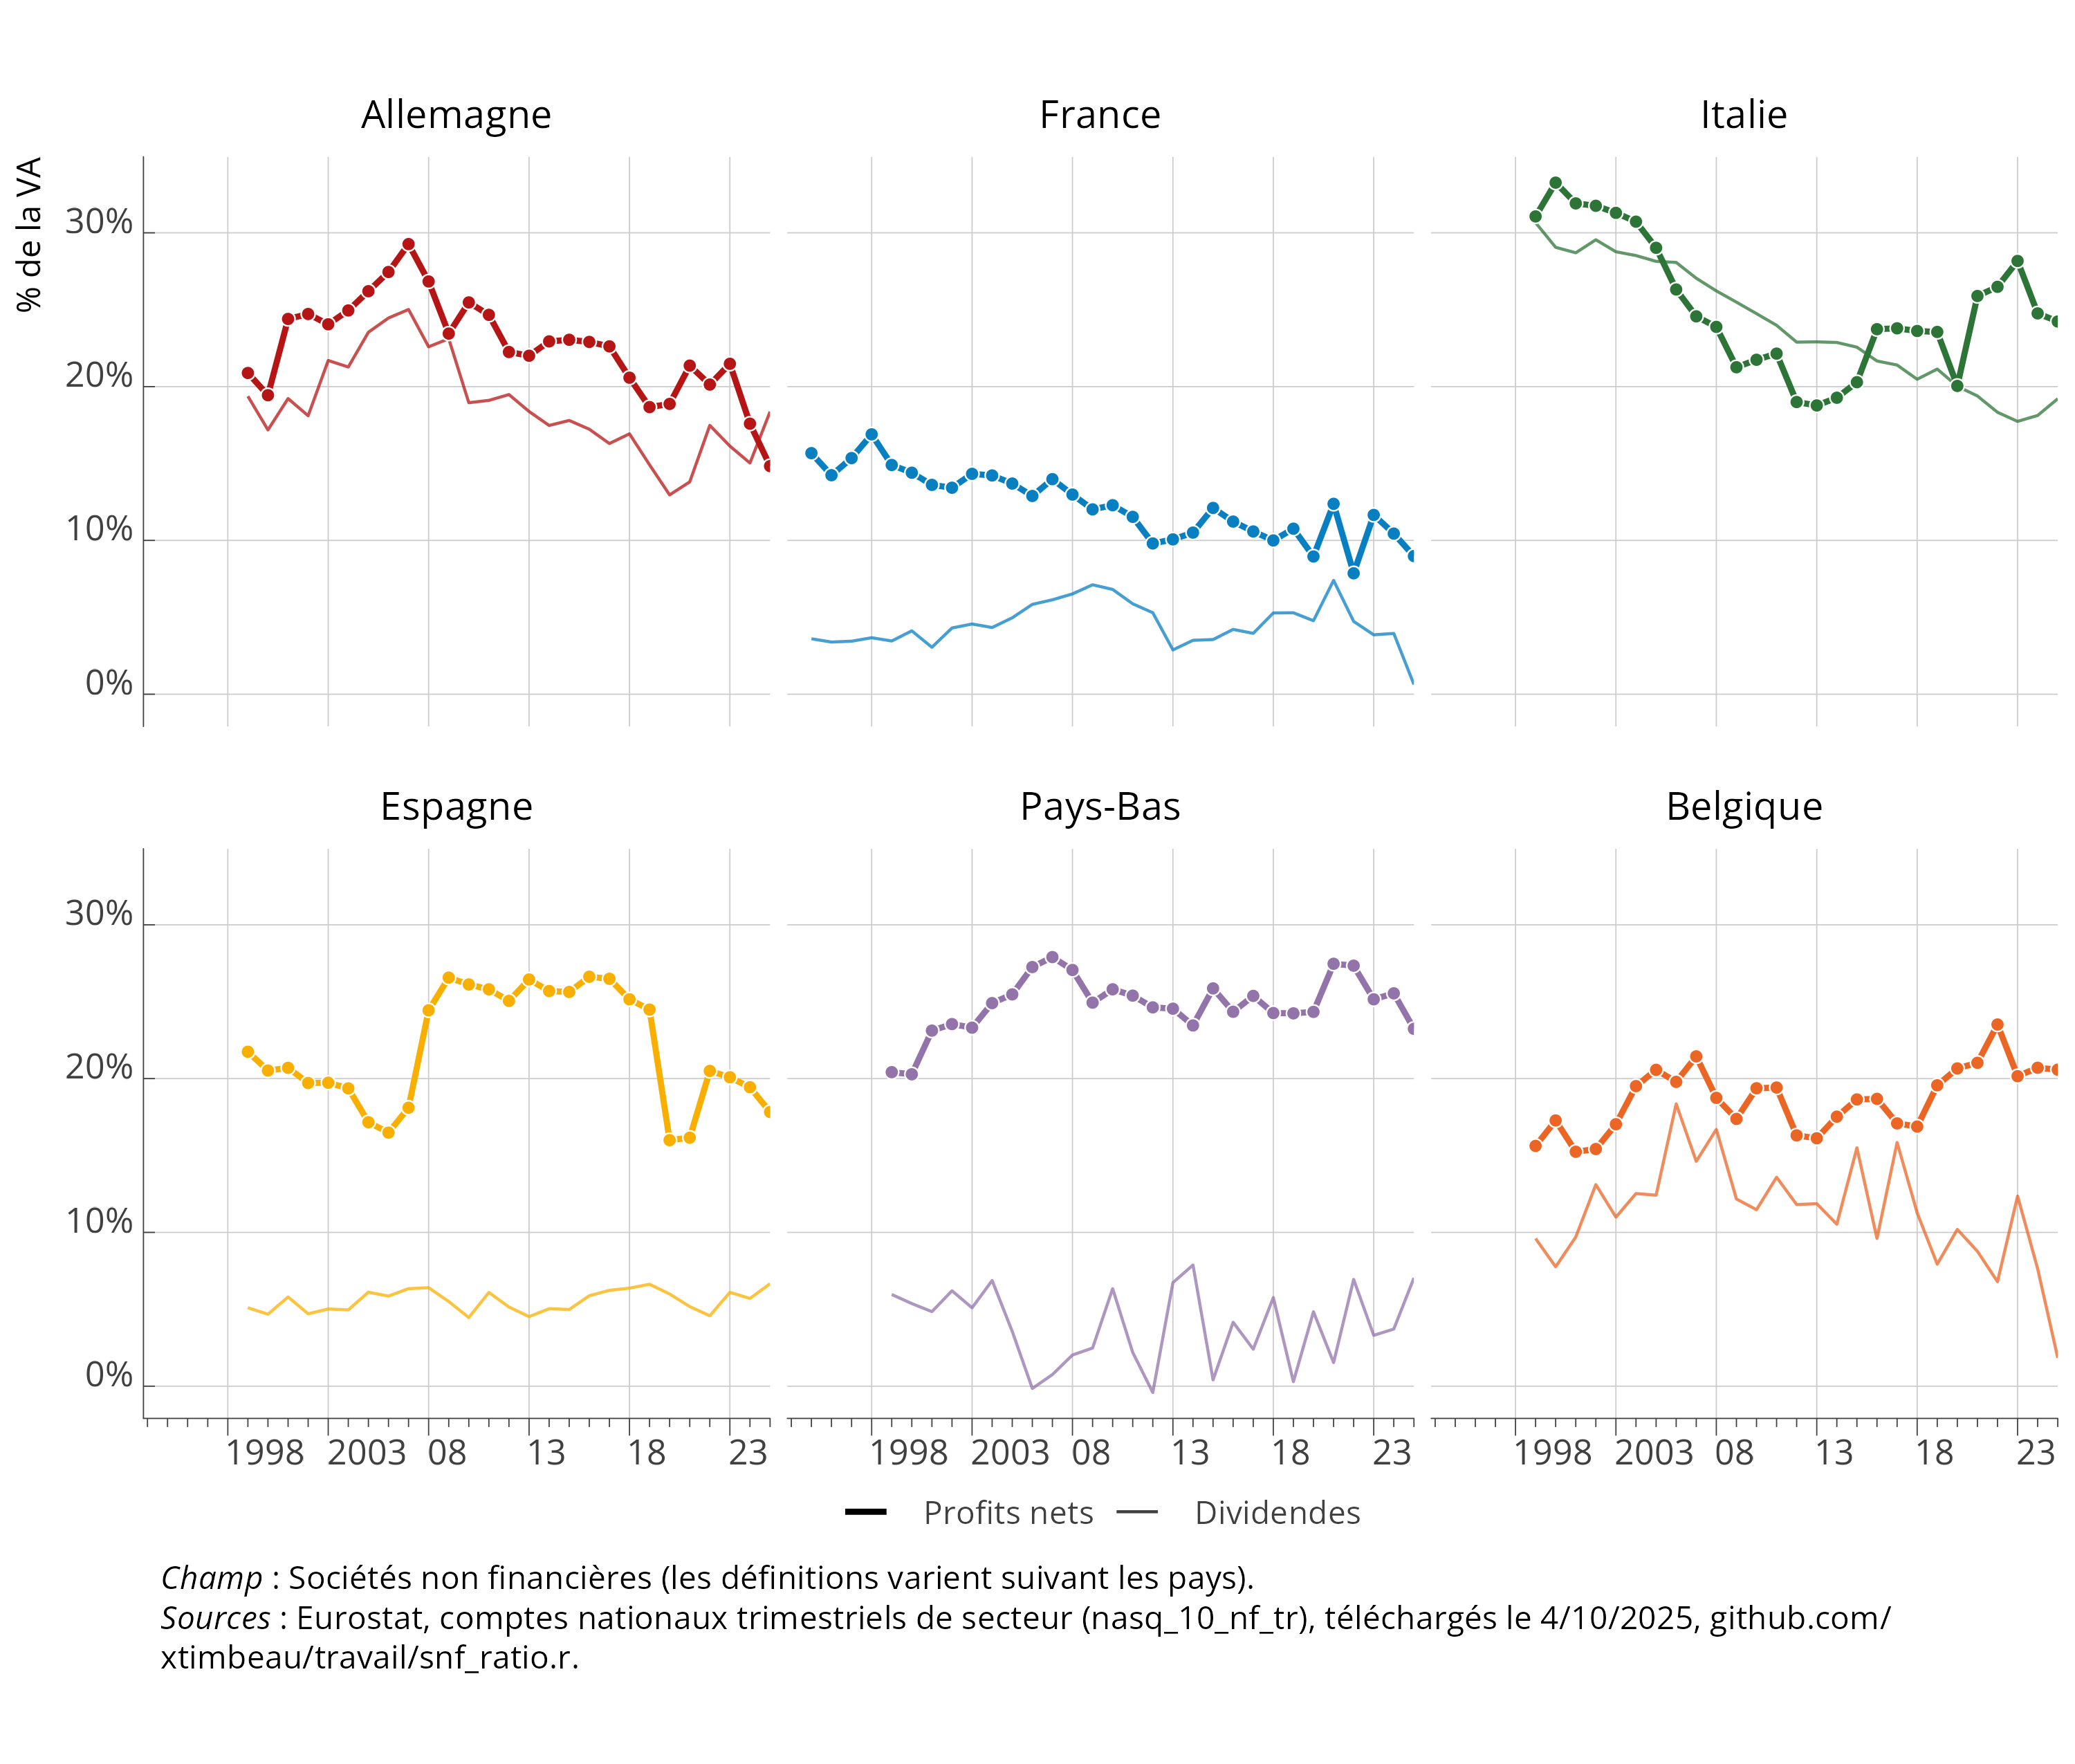
\includegraphics[width=1\linewidth,height=\textheight,keepaspectratio]{psal_comp_files/figure-pdf/fig-profits-1.png}

}

\end{figure}%

On peut rapporter ces notions aux éléments qui viennent du compte de
capital. Le premier concept est le profit rapporté au stock de capital
physique (tel que valorisé dans la comptabilité nationale, c'est-à-dire
à la valeur de remplacement et au prix de marché). Malheureusement, à
part la France, aucun pays dans notre échantillon ne diffuse ces données
sur Eurostat.

On rapporte également à une notion financière, à savoir la valeur nette
des actions au passif des comptes d'entreprises. Les conventions de
valorisation des actions non cotées sont délicates et difficiles à
suivre d'un pays à l'autre. On choisit ici d'augmenter ces actions de la
valeur nette résiduelle des entreprises non financières (\(BF90\)). On a
donc\,:

\[
\begin{aligned}
r_{productif} & = \frac{\Pi}{N1N+N2N} \\
r_{financier} & = \frac{\Pi}{F51+F52+BF90}
\end{aligned}
\]

On obtient le graphe suivant\,:

\begin{figure}[H]

\caption{\label{fig-tprofitsnff}Rendements du capital, compte de
secteur}

\centering{

\subcaption{\label{fig-tprofitsnff-1}Rendements du capital, compte de
secteur SNF}

\centering{

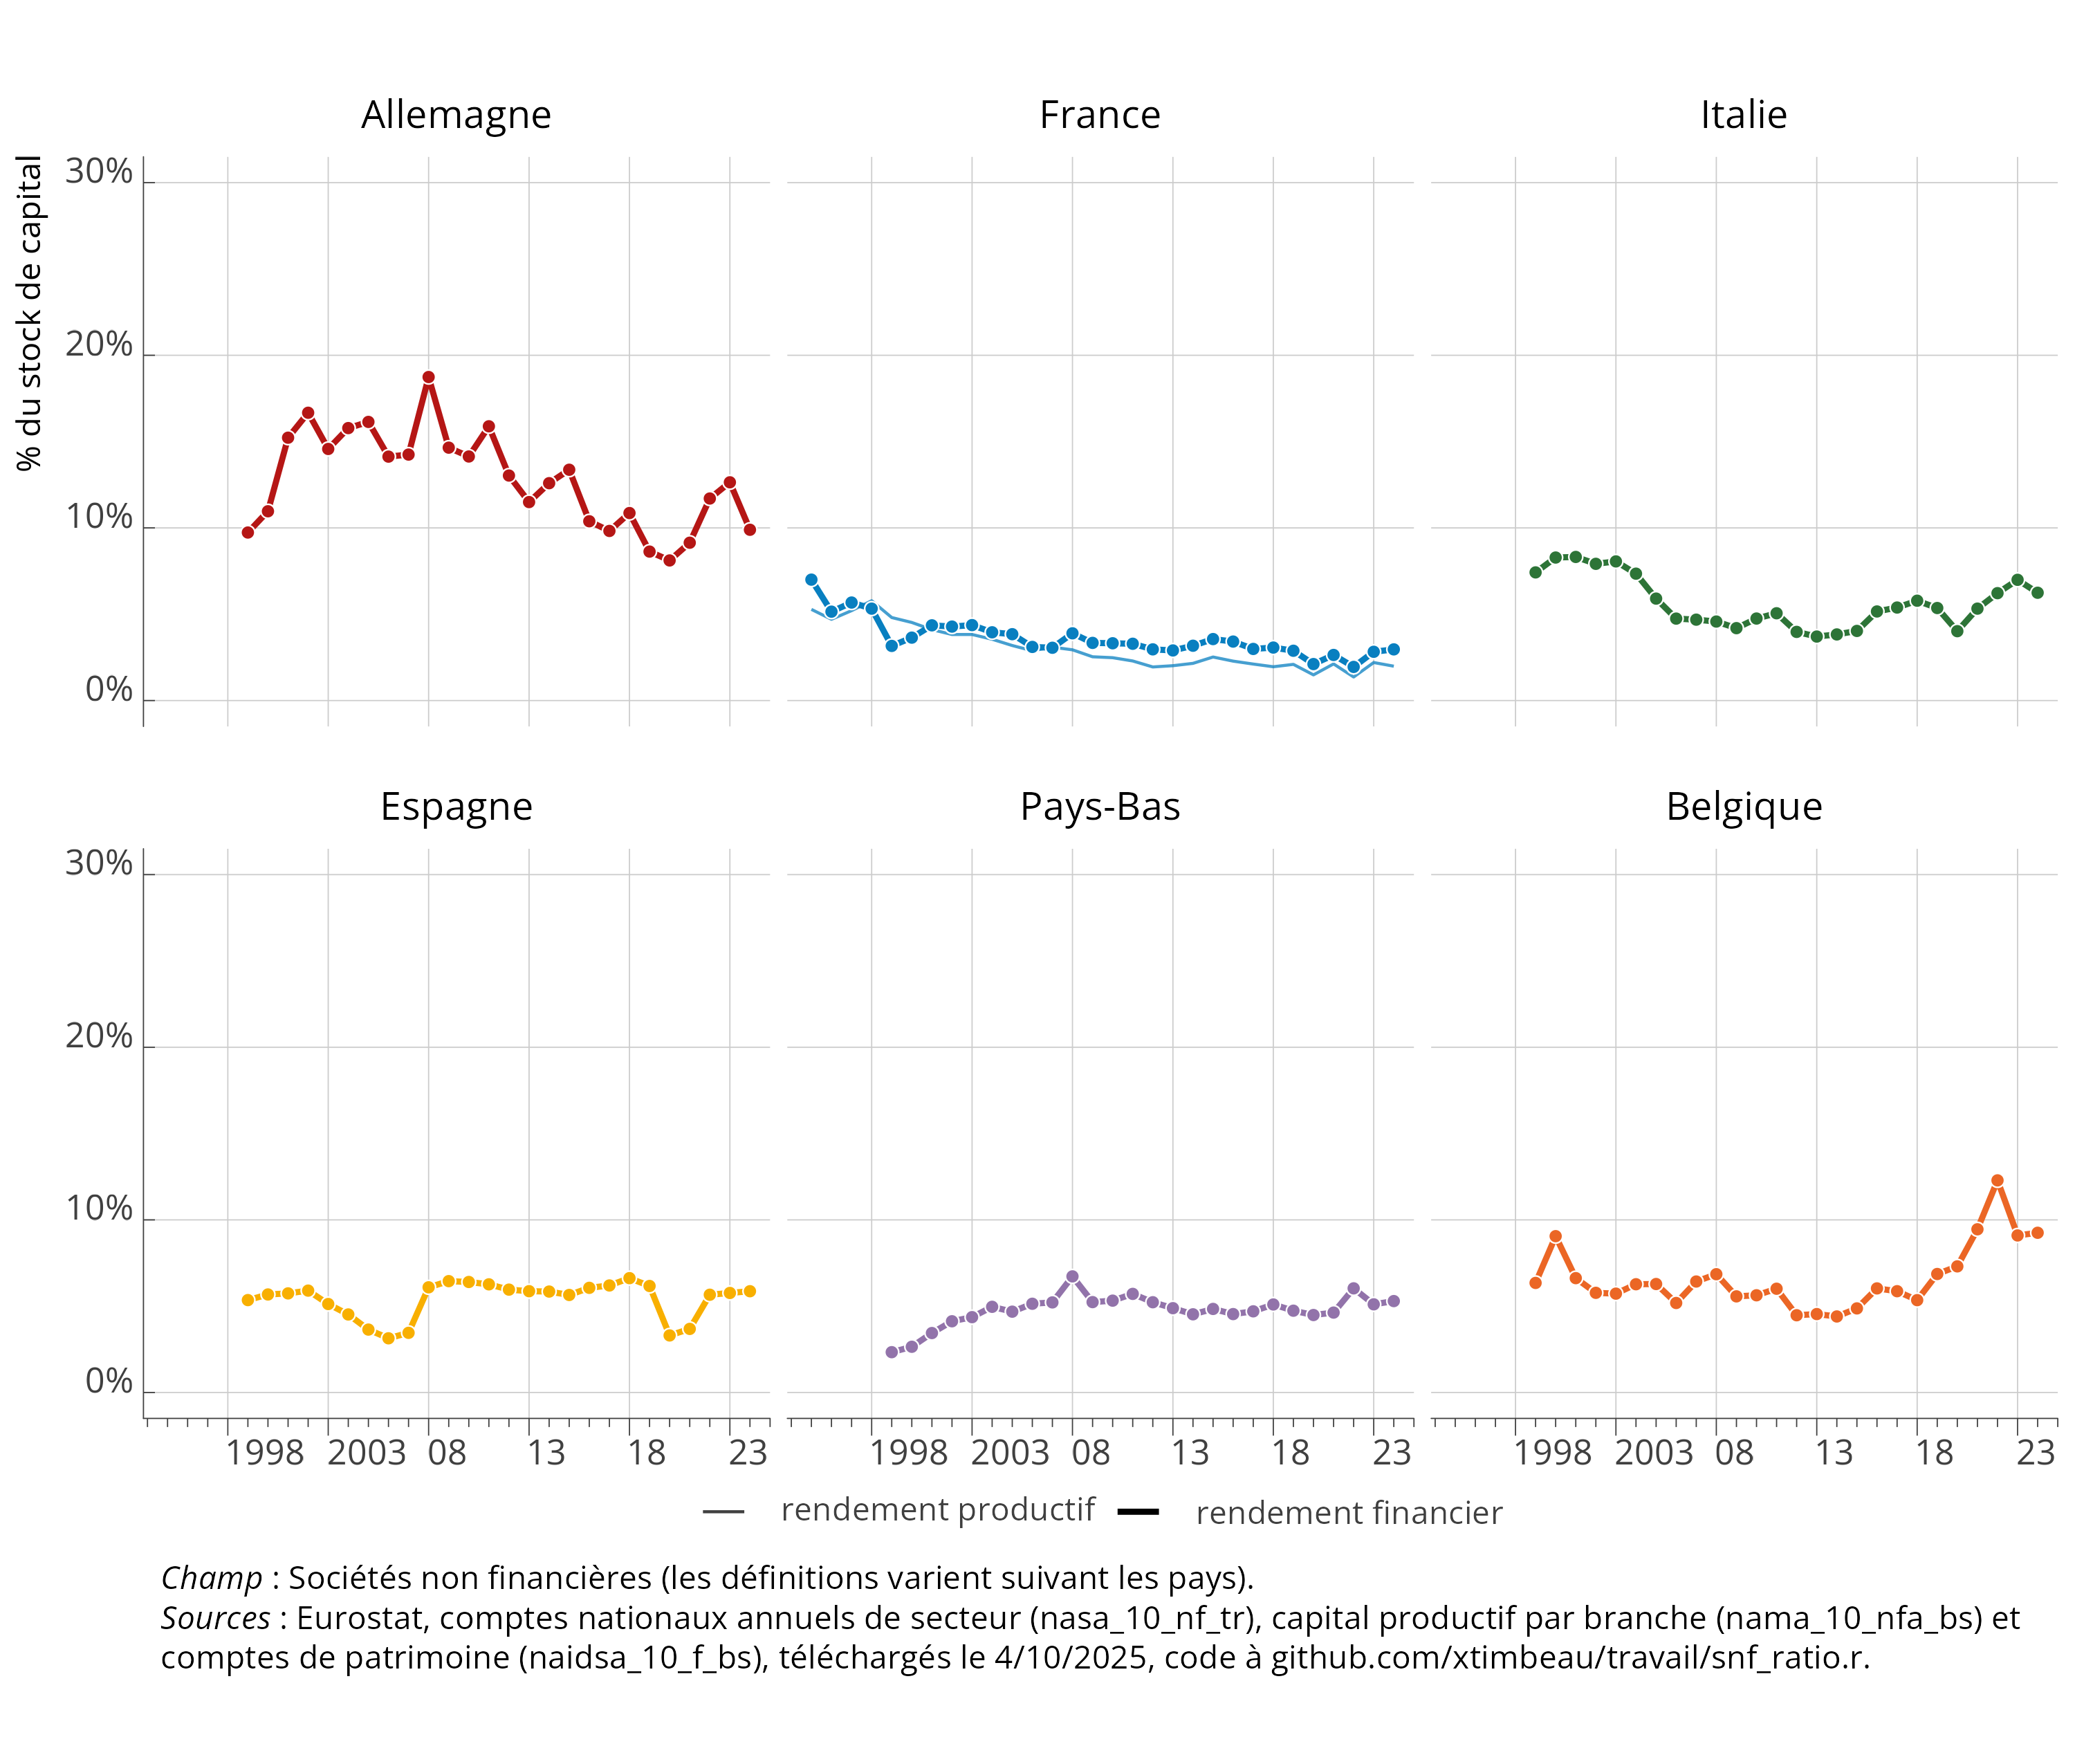
\includegraphics[width=1\linewidth,height=\textheight,keepaspectratio]{psal_comp_files/figure-pdf/fig-tprofitsnff-1-1.png}

}

}

\end{figure}%

\section{Profits nets dans les comptes de
branche}\label{profits-nets-dans-les-comptes-de-branche}

En utilisant d'une part la valeur ajoutée des branches marchandes hors
services immobiliers produits par les ménages et la valeur des actifs
productifs issue de la base des stocks de capital productif
(\href{https://ec.europa.eu/eurostat/databrowser/view/NAMA_10_NFA_ST__custom_2046386/default/table?lang=en}{nama\_10\_nfa\_st})
sur le même champ (i.e.~en enlevant la sous branche L68A), on peut
estimer un rendement du capital productif.

\begin{figure}[H]

\caption{\label{fig-tprofitbranches}Rendements du capital, compte de
branches, marchand hors services immobiliers produits par les ménages}

\centering{

\subcaption{\label{fig-tprofitbranches-1}Rendements du capital, compte
de branches, marchand hors services immobiliers produits par les ménages
Marchand-L68A}

\centering{

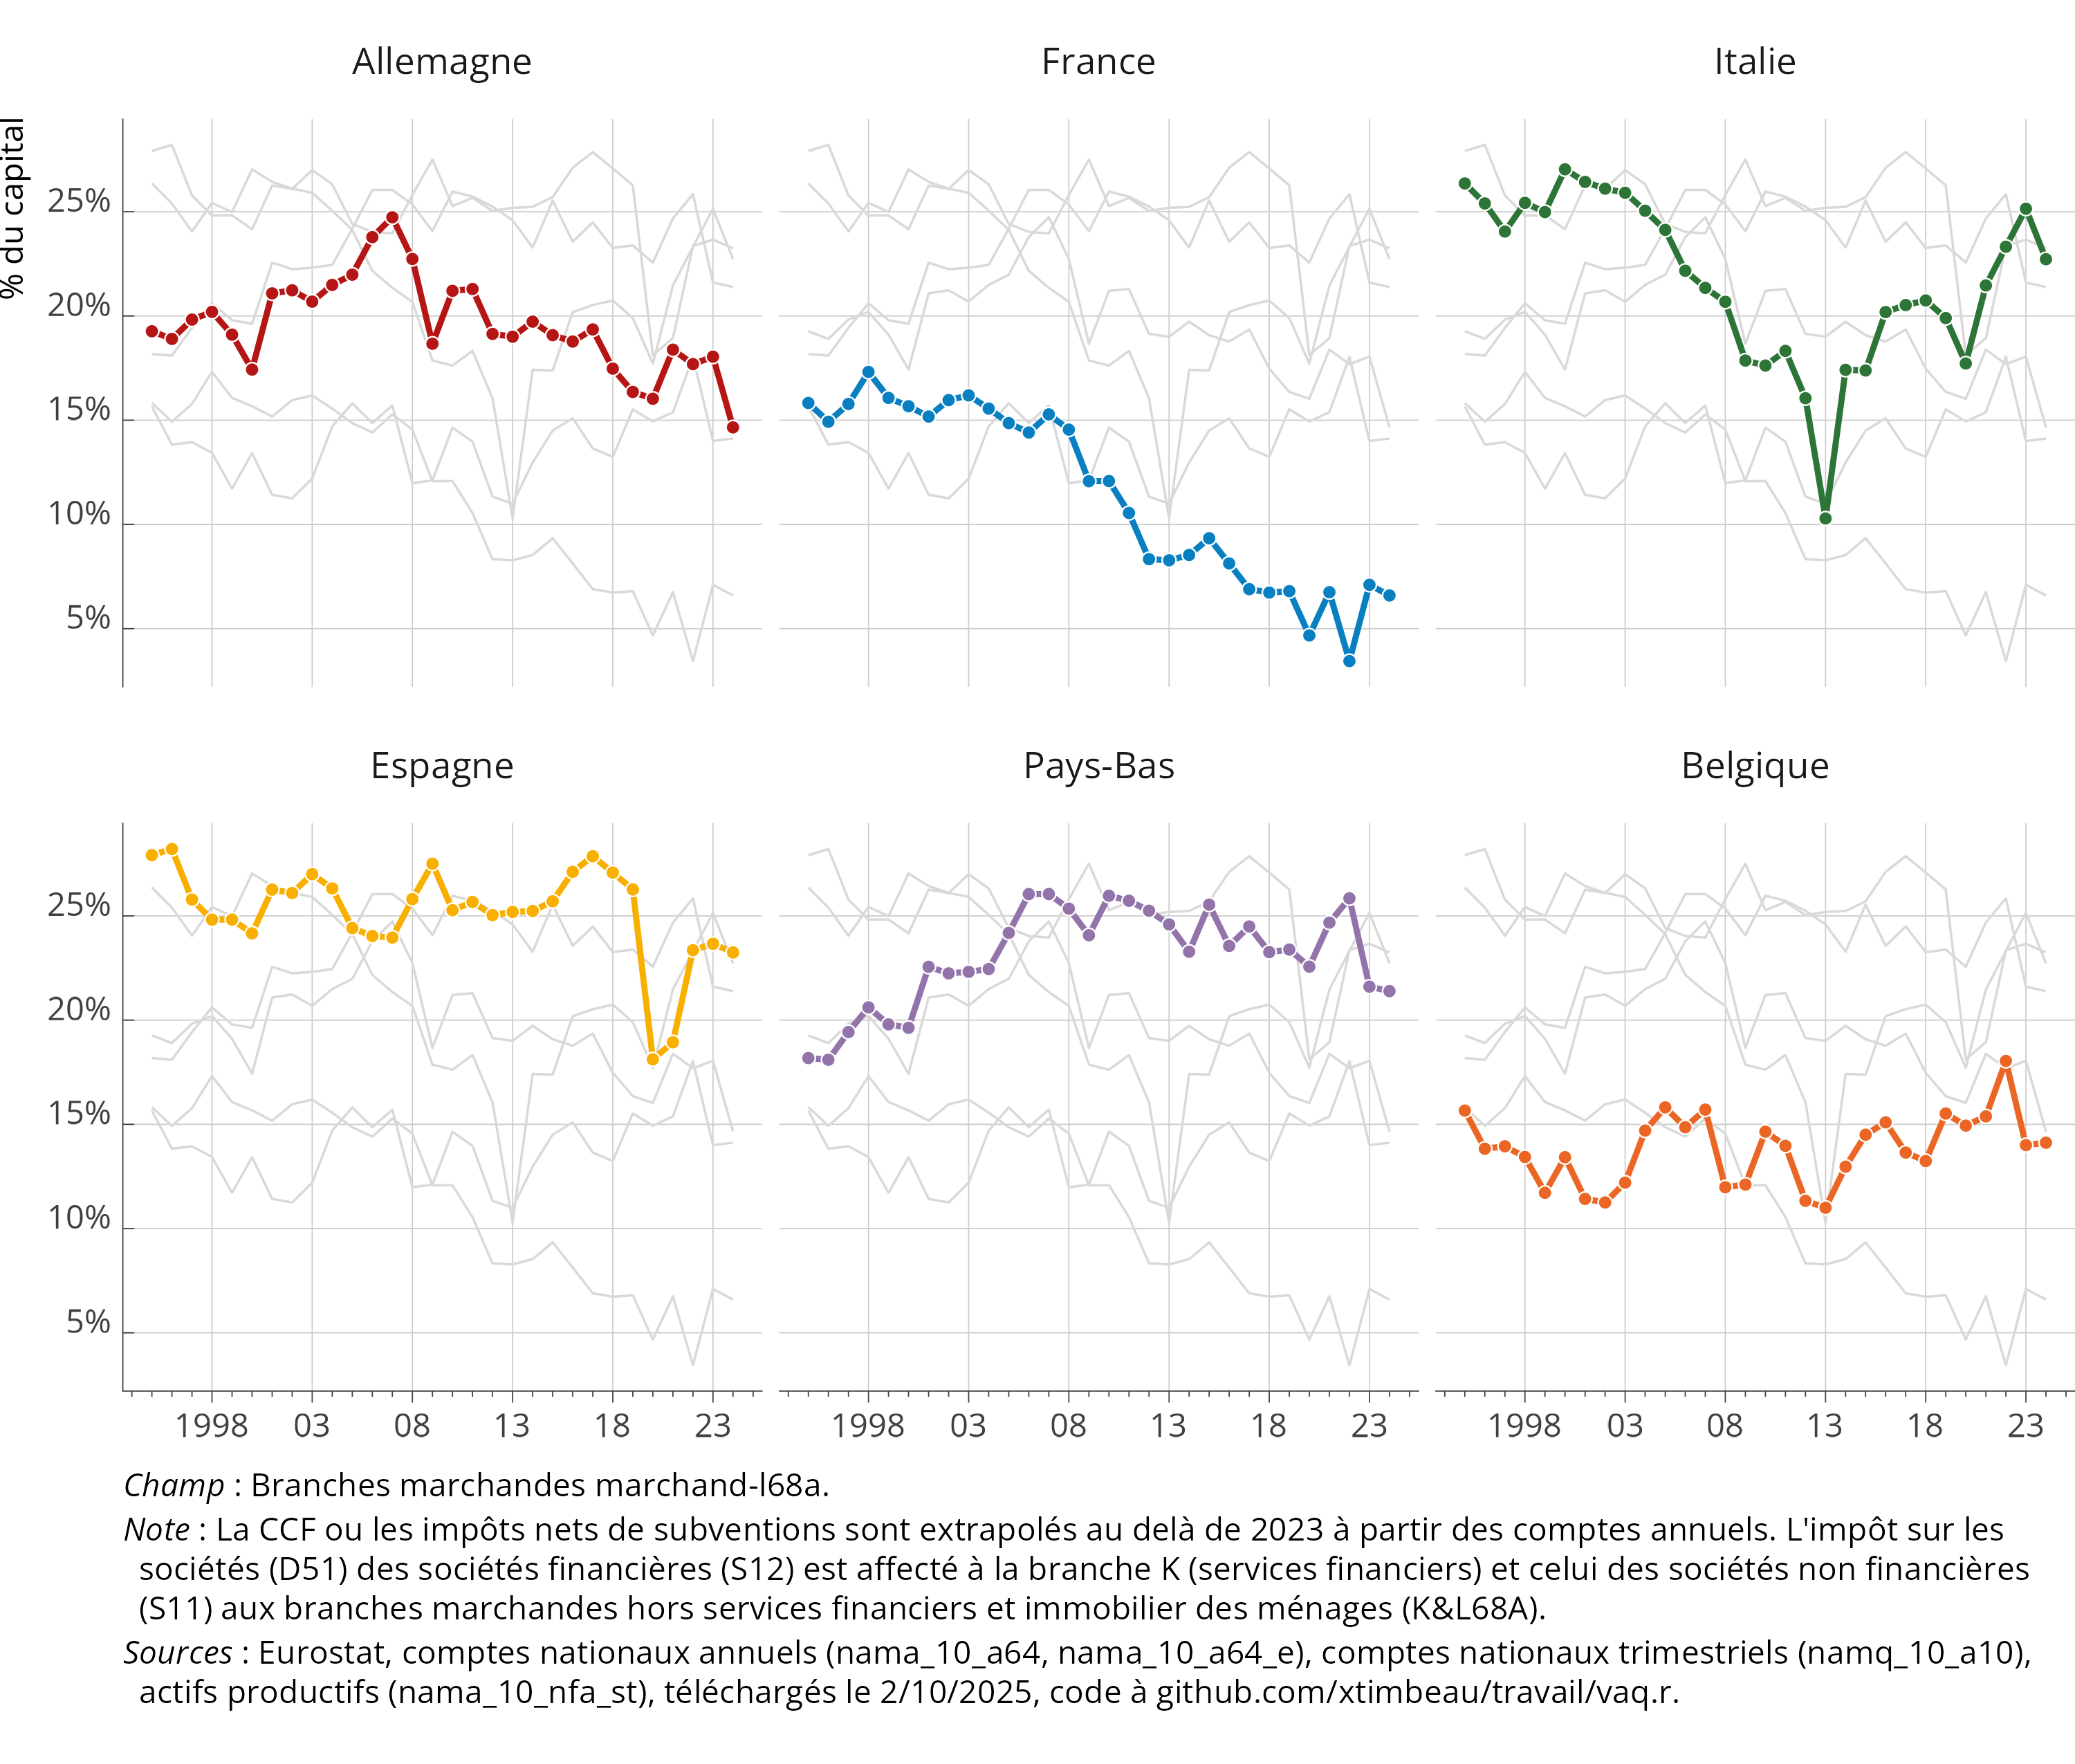
\includegraphics[width=1\linewidth,height=\textheight,keepaspectratio]{psal_comp_files/figure-pdf/fig-tprofitbranches-1-1.png}

}

}

\end{figure}%

Le rendement calculé sur le graphique~\ref{fig-tprofitbranches} diffère
de celui du graphique~\ref{fig-tprofitsnff}. La différence vient en
partie de la difficulté à imputer l'impôt des sociétés aux seules
entreprises des branches marchandes\,-- des entités légales dans les
branches non marchandes peuvent être soumises à l'impôt sur les sociétés
et de la valorisation des actifs. Dans l'approche comptes d'agents (ou
de secteurs institutionnels), on affecte la valeur nette résiduelle des
entreprises au stock de capital. De plus, le stock de capital n'est pas
dans l'approche du graphique~\ref{fig-tprofitsnff} limité au capital
productif mais intègre également des actifs financiers qui n'ont pas de
contrepartie physique parce qu'ils sont hors territoire français.

La France conserve une singularité marquée par la baisse continue du
taux de profit au cours du temps. Le rendement apparent du capital est
ainsi très bas, plus bas que dans tous les autres pays considérés où il
est plutôt stable (l'Italie fait exception avec une forte volatilité).

\section{Au delà de l'Europe}\label{au-deluxe0-de-leurope}

L'accès aux données de l'OCDE est devenu particulièrement opaque, mais
je m'en suis sorti. Il est possible d'utiliser des données de
comptabilité nationale, au niveau de l'ensemble de l'économie (y compris
donc les branches non marchandes et l'immobilier). La correction pour la
non-salarisation est assurée par les données de l'\emph{Economic
Outlook} (avec une trimestrialisation \emph{ad hoc}). Au lieu de la
valeur ajoutée, on utilise le PIB, auquel on enlève la consommation de
capital fixe (dans les données OCDE, il n'y a pas de données de CCF pour
le Japon). Le concept de part des salaires n'est donc pas tout à fait le
même que dans les autres analyses.

On obtient ce graphique\,:

\begin{figure}[H]

\caption{\label{fig-psaloecd}Part des salaries dans le PIN, données SNA
de l'OCDE}

\centering{

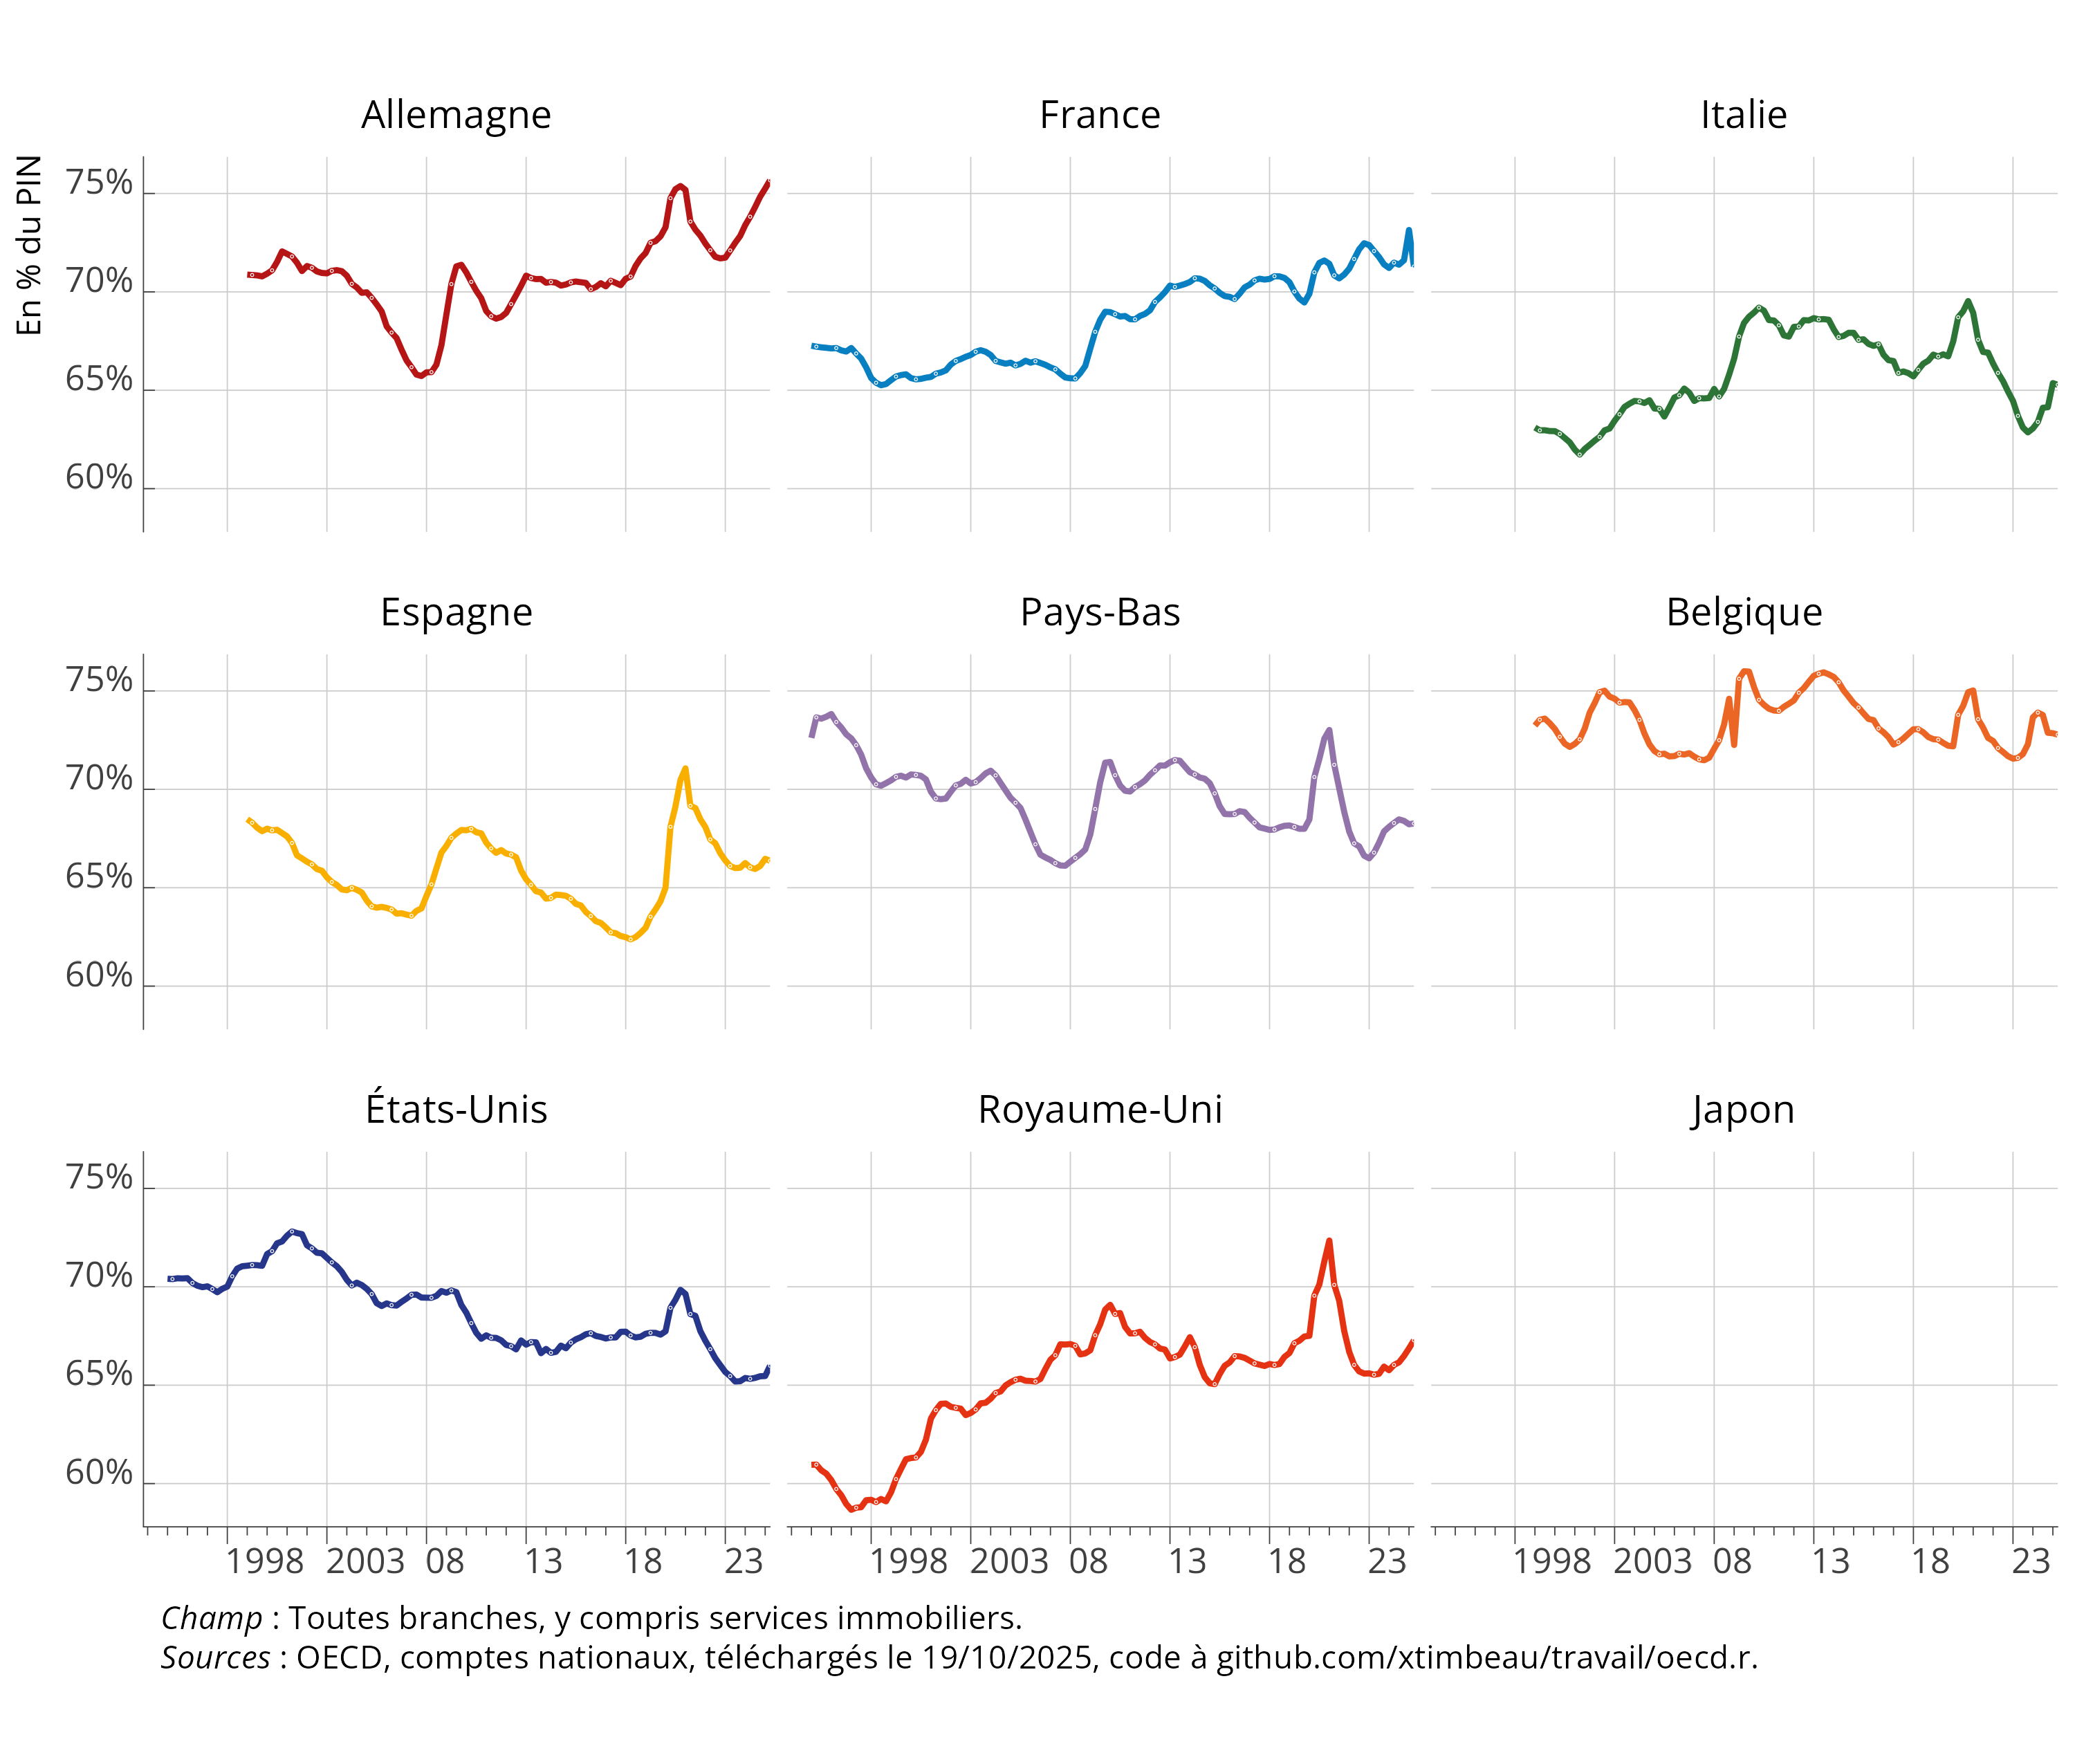
\includegraphics[width=1\linewidth,height=\textheight,keepaspectratio]{psal_comp_files/figure-pdf/fig-psaloecd-1.png}

}

\end{figure}%

En revanche, Eurostat a un programme de coopération (avec l'OCDE) pour
intégrer les données dans le cadre d'Eurostat (sans que les méthodes ne
soient plus homogènes pour autant).

On utilise ces données
(\href{https://ec.europa.eu/eurostat/databrowser/view/naidsa_10_nf_tr__custom_13241966/default/table?lang=en}{\texttt{naidsa\_10\_nf\_tr}})
pour construire des indicateurs comparables en comparant des pays autres
que ceux de la zone euro.

\begin{figure}[H]

\caption{\label{fig-tprofithze}Part des salaires dans la valeur ajoutée,
comptes de secteur, comparaisons internationales}

\centering{

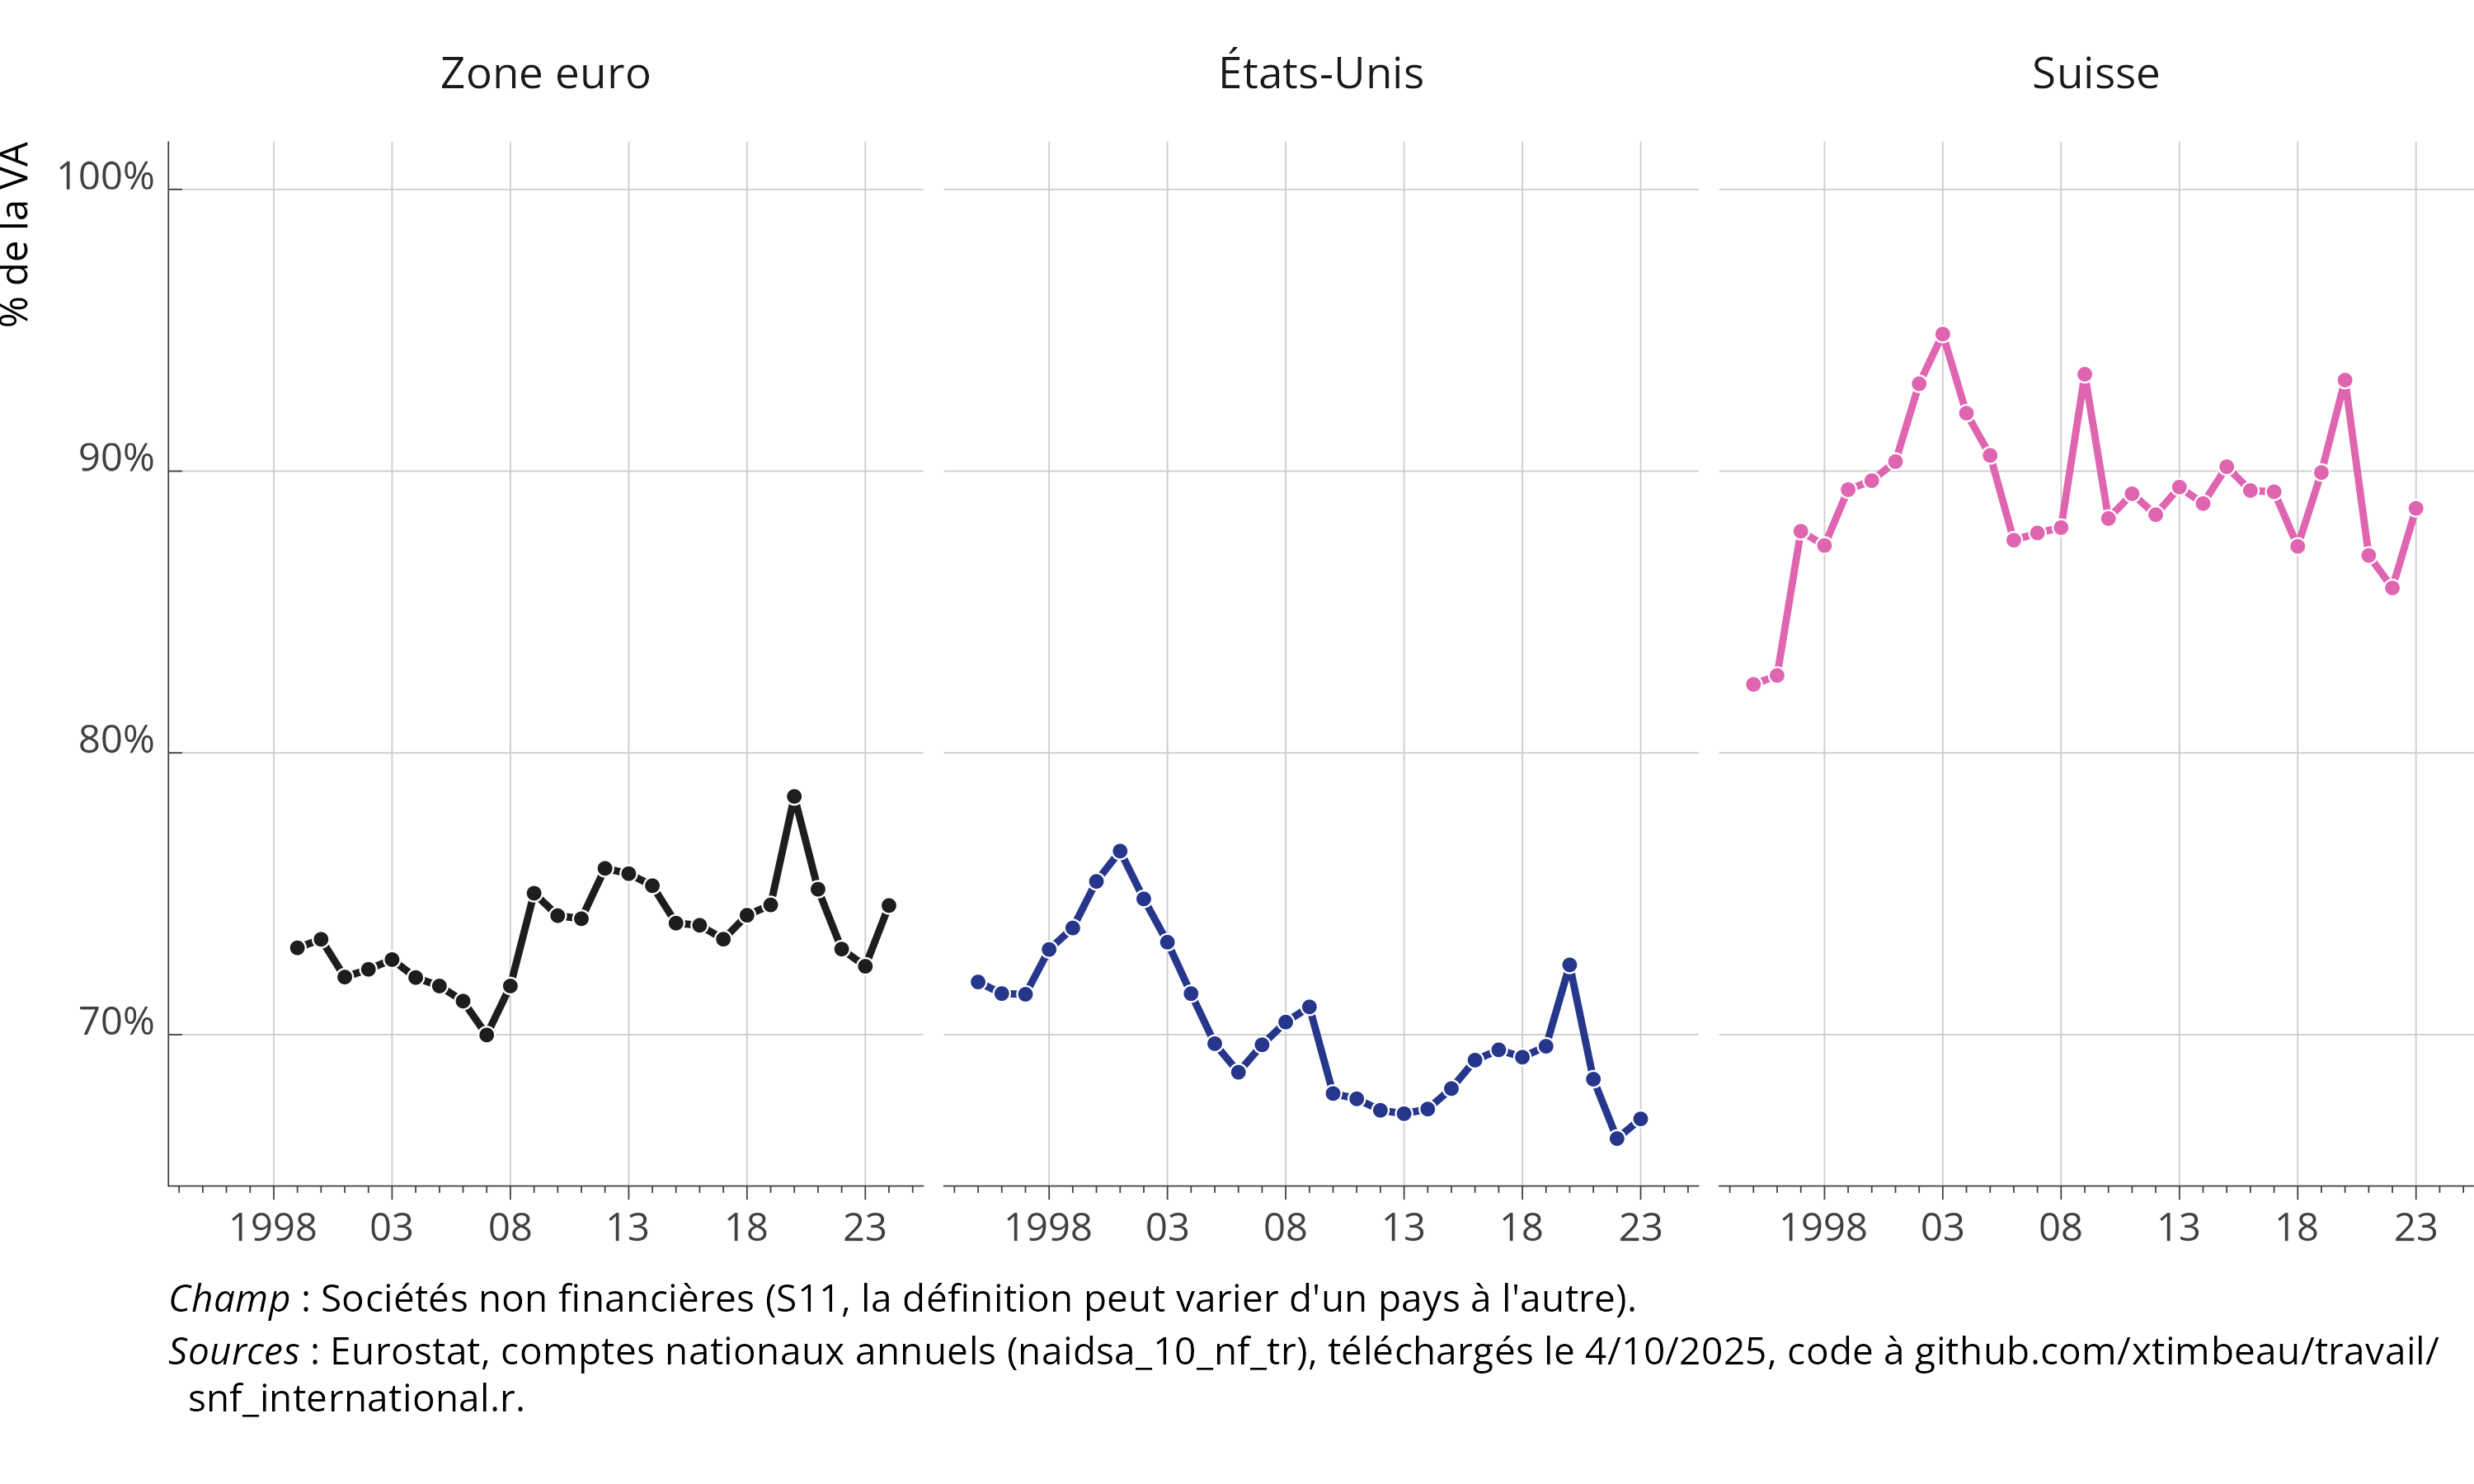
\includegraphics[width=1\linewidth,height=\textheight,keepaspectratio]{psal_comp_files/figure-pdf/fig-tprofithze-1.png}

}

\end{figure}%

\subsection*{Références}\label{ruxe9fuxe9rences}

\phantomsection\label{refs}
\begin{CSLReferences}{0}{1}
\bibitem[\citeproctext]{ref-askenazy2012}
Askenazy P., Cette G., Sylvain A. (2012).
{«~\href{https://doi.org/10.3917/dec.asken.2012.01}{Le partage de la
valeur ajoutée}~»}, \emph{Repères}.

\bibitem[\citeproctext]{ref-cotis2009}
Cotis J.-P. (2009).
{«~\href{https://www.vie-publique.fr/rapport/30455-partage-valeur-ajoutee-partage-profits-et-ecarts-de-remuneration}{Partage
de la valeur ajoutée, partage des profits et écarts de rémunérations en
France}~»}, Présidence de la République Française.

\bibitem[\citeproctext]{ref-hurlin1996}
Hurlin C., Portier F. (1996).
{«~\href{https://doi.org/10.3406/ecop.1996.5809}{Le partage de la valeur
ajoutée dans le cycle}~»}, \emph{Économie \& prévision}, \emph{125}, n°
4, p.~73‑85.

\bibitem[\citeproctext]{ref-husson2010}
Husson M. (2010). {«~\href{https://doi.org/10.3917/rdli.064.0047}{Le
partage de la valeur ajoutée en Europe}~»}, \emph{La Revue de l'Ires},
\emph{n° 64}, n° 1, p.~47‑91.

\bibitem[\citeproctext]{ref-piton2019}
Piton S. (2019). {«~\href{https://doi.org/10.3917/rce.024.0131}{7. Le
partage de la valeur ajoutée~n{'}a pas encore dévoilé tous ses
mystères}~»}, \emph{Regards croisés sur l'économie}, \emph{n° 24}, n° 1,
p.~131‑140.

\bibitem[\citeproctext]{ref-timbeau2002}
Timbeau X. (2002). {«~\href{https://doi.org/10.3917/reof.080.0063}{Le
partage de la valeur ajoutée en France}~»}, \emph{Revue de l'OFCE},
\emph{80}, n° 1, p.~63.

\bibitem[\citeproctext]{ref-timbeau2025}
Timbeau X. (2025).
{«~\href{https://shs.cairn.info/revue-l-economie-politique-2025-1-page-64?lang=fr}{Quelles
marges de manœuvre pour revaloriser le travail ?}~»}, \emph{Economie
Politique}, \emph{105}, n° 1, p.~64‑75.

\bibitem[\citeproctext]{ref-tuxf8rsluxf8v2022}
Tørsløv T., Wier L., Zucman G. (2022).
{«~\href{https://doi.org/10.1093/restud/rdac049}{The Missing Profits of
Nations}~»}, \emph{The Review of Economic Studies}, \emph{90}, n° 3,
p.~1499‑1534.

\end{CSLReferences}




\end{document}
